\documentclass[11pt,a4paper]{article}

\usepackage[margin=1in]{geometry}
\usepackage{authblk}
\usepackage{amsmath,amssymb,amsfonts}
\usepackage{graphicx}
\usepackage{booktabs}
\usepackage{placeins}
\usepackage{hyperref}
\usepackage{url}
\usepackage{xurl}
\usepackage{cite}
\usepackage{caption}
\usepackage{tikz}
\usepackage{pgfplots}
\usepgfplotslibrary{groupplots}
\pgfplotsset{compat=1.17}

\hypersetup{
    colorlinks=true,
    linkcolor=blue,
    citecolor=blue,
    urlcolor=blue
}

\title{\textbf{Pitfalls of Single-Metric Evaluation for Quantized Reasoning Checkpoints}}

\author[1,2]{Manish Nandish}
\author[1]{Rajiv Misra}
\author[2]{Midhunchakkaravarthy Janarthanan}
\affil[1]{Department of Computer Science and Engineering, Indian Institute of Technology Patna, Patna, Bihar, India\\
\texttt{manish\_25s21res58@iitp.ac.in}, \texttt{rajivm@iitp.ac.in}}
\affil[2]{Lincoln University College, Malaysia\\
\texttt{midhun@lincoln.edu.my}}
\renewcommand\Affilfont{\normalsize\itshape}

\date{23 September 2026}

\begin{document}

\maketitle

\begin{abstract}
Practitioners often select a public quantized reasoning checkpoint from a single metric. We pin one A100 stack (vLLM~0.7.0 eager~\cite{kwon2023vllm}) and evaluate eight DeepSeek-R1-Distill checkpoints---Qwen-7B and Llama-8B, in BF16, Marlin W8A16 FP8~\cite{frantar2024marlin}, community AWQ-4, and RedHatAI GPTQ-4---on MATH-500~\cite{hendrycks2021math,lightman2023lets}, GSM8K~\cite{cobbe2021gsm8k}, and GPQA-Diamond~\cite{rein2023gpqa} (88 runs, 56{,}408 completions).

The robust accuracy drop is Llama AWQ-4 (MATH-500 $-2.76$\,pp; GSM8K $-1.57$\,pp). maj@5 cuts that MATH gap to about $-1.4$\,pp and removes the smaller Qwen AWQ-4 gap. A BF16-correct length contrast is positive in every cell because it includes quantized failures; the mirrored quant-correct contrast flips sign in four of six cells, and three of those intervals exclude zero. Subset serving cost is dominated by one length draw: Llama FP8 averages about $7{,}288$ tokens on the 20-prompt Condition~A subset and $4{,}551$ on the full grid, and timing repeats do not resample that draw. Gold-free 5/5 agreement has selective risk at most $0.27\%$, against $1.6$--$4.6\%$ for a one-sample length rule at matched coverage.
\end{abstract}

\vspace{0.6em}
\noindent\textbf{Keywords:} Reasoning language models, quantization checkpoints, selection effects, majority vote, selective prediction.

\section{Introduction}
Reasoning models such as DeepSeek-R1~\cite{guo2025deepseekr1} emit long traces before a final answer. Post-training quantization (FP8, AWQ-4~\cite{lin2023awq}, GPTQ-4~\cite{frantar2022gptq}) is a common serving choice, and practitioners often pick a public checkpoint from a single published pass@1. Isolated pass@1 numbers hide whether the same checkpoint also changes trace length~\cite{lian2026quantinflates,liu2025qrm,lotfi2026overthinking}, termination, or the cost of a correct answer~\cite{erol2025costofpass,kurtic2025give}. Serving-stack details---engine version, decoding flags, CUDA graphs---can materially move reasoning scores~\cite{hochlehnert2025sober}. This paper \emph{pins} one stack rather than shifting it: we do not run a factorial vLLM $0.7.0$ vs.\ $0.8.5$ experiment. The unit of analysis is the public checkpoint $\times$ pinned serving stack $\times$ evaluation target.

We ask four questions under that pin:
\begin{itemize}
    \item \textbf{RQ1.} Which pass@1 differences survive an item-level interval, and how much of a 4-bit gap does maj@5 remove?
    \item \textbf{RQ2.} Is a BF16-correct length increase a property of the checkpoint, or a selection effect of conditioning on quantized failures?
    \item \textbf{RQ3.} At matched coverage, does five-sample answer agreement have lower selective risk than a one-sample length rule?
    \item \textbf{RQ4.} How much of a subset serving-cost gap is one length draw that timing repeats do not cover?
\end{itemize}

\noindent\textbf{Contributions.}
(C1)~\textbf{Selection effect in the BF16-correct length estimator.} The Lian-style conditional is positive in every contrast. Its quant-correct mirror flips sign in four of six contrasts. Both columns are selection effects, not a reconciliation of prior length claims.
(C2)~\textbf{Subset serving cost is a length draw.} Timing repeats share one sampling seed. Campaign-length seconds, using the same measured tok/s, put Llama FP8 first on both conditions in all $10{,}000$ item resamples. The 20-prompt Condition~A order does not.
(C3)~\textbf{One robust accuracy drop, and a gold-free check.} Llama AWQ-4 is the Holm-significant MATH and GSM8K drop. maj@5 recovers most of it. Five-sample agreement beats a one-sample length rule on selective risk at matched coverage. AWQ results are properties of the \texttt{jakiAJK} artifacts run in \texttt{float16} on the GEMM \texttt{awq} kernel, not a property of the AWQ method.

\section{Related Work}
GPTQ~\cite{frantar2022gptq} and AWQ~\cite{lin2023awq} were originally validated mainly on short-form benchmarks. Liu et al.\ (QRM; COLM 2025)~\cite{liu2025qrm} evaluate DeepSeek-R1 distillations across weight, activation, and KV quantization, reporting accuracy and mean length. Kurtic et al.~\cite{kurtic2025give} study vLLM serving efficiency across formats and batching regimes. Lian et al.~\cite{lian2026quantinflates} isolate token inflation on BF16-correct traces. Hochlehnert et al.~\cite{hochlehnert2025sober} show that seeds, prompts, decoding, and software move reasoning scores. Erol et al.~\cite{erol2025costofpass} define Cost-of-Pass as expected monetary cost per correct solution.

Existing studies evaluate quantization accuracy, throughput, or individual reasoning behaviors. Kurtic et al.\ already show that format recommendations change between synchronous decode and continuous batching. Our Condition~A versus Condition~B contrast is a pinned-stack sensitivity on these public checkpoints, not a second batching law. Appendix Table~\ref{tab:economics} reports mean tokens divided by pass@1. Appendix Table~\ref{tab:related} places this grid against those studies. The unit of comparison is the public checkpoint $\times$ pinned stack $\times$ evaluation target.

\begin{table}[t]
\centering
\caption{Qwen-7B numbers reported by QRM beside this pinned grid. Cells are matched by benchmark and format. The GPQA row is not a certified paired contrast (Appendix Section~\ref{sec:prompt}). The discrepancy is checkpoint- and stack-sensitive measurement, not a superiority claim.}
\label{tab:qrm-compare}
\small
\begin{tabular}{lcc}
\toprule
\textbf{Cell} & \textbf{QRM} & \textbf{This grid} \\
\midrule
MATH-500 BF16 & 94.60 & 94.00 \\
MATH-500 AWQ-4 & 91.00 & 93.12 \\
GPQA-Diamond AWQ-4 & 50.00 & 44.78 \\
\bottomrule
\end{tabular}
\end{table}

The FP8 and GPTQ-4 cells are public RedHatAI compressed-tensors checkpoints evaluated as A100 Marlin weight-only kernels. These are not Red Hat production-deployment measurements. We do not rerun SmoothQuant~\cite{xiao2023smoothquant}. Lotfi et al.~\cite{lotfi2026overthinking}, Li et al.~\cite{li2025quantmeets}, Helcig et al.~\cite{helcig2026slq}, Zhong et al.~\cite{zhong2025quantized}, and Ayadi et al.~\cite{ayadi2026reliability} study overthinking, reasoning degradation, statistically lossless quantization, calibration, and reliability scaling; we do not re-estimate those quantities. Self-consistency~\cite{wang2022selfconsistency} and G-Pass@$k$~\cite{liu2025gpass} are different estimands from the unique-mode rule in Section~\ref{sec:modal}. We report mean tokens divided by pass@1, and an aggregate hybrid Cost-of-Pass proxy from measured GPU-seconds; neither is Erol et al.'s per-problem estimator.

\section{Experimental Methodology}
\subsection{Models and precision formats}
We evaluate DeepSeek-R1-Distill-Qwen-7B and DeepSeek-R1-Distill-Llama-8B~\cite{guo2025deepseekr1}. Formats: uncompressed \textbf{BF16}; \textbf{FP8} checkpoints served on A100 via vLLM's Marlin \textbf{W8A16} weight-only fallback (not native W8A8 tensor-core FP8); \textbf{AWQ-4} (group size 128); \textbf{GPTQ-4} (group size 128). Hugging Face IDs and revisions are in Appendix Table~\ref{tab:checkpoints}. Table~\ref{tab:dtype} records the activation dtype and kernel. An AWQ-versus-BF16 contrast is therefore quantization plus a change from \texttt{bfloat16} to \texttt{float16} activations. Qwen-family models have a known \texttt{float16} overflow history; this grid does not include a BF16 checkpoint rerun at \texttt{dtype=float16}, so that mechanism is not identified. Accuracy-campaign GPTQ-4 stays on \texttt{bfloat16}. The serving script sets \texttt{float16} for both AWQ-4 and GPTQ-4, so the GPTQ accuracy cells and the GPTQ timing cells do not share an activation dtype.

\subsection{Benchmarks and protocol}
MATH-500~\cite{hendrycks2021math,lightman2023lets} ($n=500$, seeds $42$--$46$): 20{,}000 completions. GSM8K~\cite{cobbe2021gsm8k} ($n=1{,}319$, seeds $42$--$44$) and GPQA-Diamond~\cite{rein2023gpqa} ($n=198$, seeds $42$--$44$): breadth. Decoding follows the QRM chat template in Appendix Section~\ref{sec:prompt}, with $T=0.6$, top-$p=0.95$, repetition penalty $1.0$ (deliberately not used to hide loops), and max new tokens $32{,}768$. Total: $56{,}408$ completions in 88 checkpoint$\times$benchmark$\times$seed runs. Throughout, a \emph{run} denotes one checkpoint$\times$benchmark$\times$seed evaluation; a \emph{cell} denotes one checkpoint$\times$benchmark aggregated over its evaluated seeds; a \emph{format contrast} compares a quantized checkpoint with its matched BF16 checkpoint within the same model family and benchmark. MATH and GSM8K are widely used; a paired within-item design reduces but does not eliminate contamination interaction with format.

\begin{table}[t]
\centering
\caption{Activation dtype and vLLM kernel. Accuracy dtype is the 56k campaign. Serving dtype is the confirmation timer. AWQ uses the GEMM awq kernel, not awq-marlin. GPTQ's checkpoint file is compressed-tensors; the kernel is Marlin W4A16. Accuracy-campaign GPTQ uses bfloat16 and the timer uses float16.}
\label{tab:dtype}
\small
\begin{tabular}{llll}
\toprule
\textbf{Format} & \textbf{Accuracy dtype} & \textbf{Accuracy kernel} & \textbf{Serving dtype} \\
\midrule
BF16 & \texttt{bfloat16} & native & \texttt{bfloat16} \\
FP8 & \texttt{bfloat16} & Marlin W8A16 & \texttt{bfloat16} \\
AWQ-4 & \texttt{float16} & GEMM \texttt{awq} & \texttt{float16} \\
GPTQ-4 & \texttt{bfloat16} & Marlin W4A16 & \texttt{float16} \\
\bottomrule
\end{tabular}
\end{table}

\subsection{Hardware and serving stack}
PARAM Rudra HPC (IIT Patna / NSM), NVIDIA A100-PCIE-80GB. Publication runs use the official QRM \texttt{inference.py} path~\cite{liu2025qrm} with \texttt{gpu\_memory\_utilization=0.75}. Engine pin: \texttt{vLLM==0.7.0}, \texttt{enforce\_eager=true}. Eager execution keeps the accuracy path reproducible and adds CPU kernel-launch overhead on single-stream decode. Production serving more often uses CUDA graphs. This paper has no CUDA-graph replicate, so Condition~A format gaps are specific to eager execution. Effective launch settings are recorded in \path{results/reports/runtime_manifest.json}.

\subsection{Measured serving}
\label{sec:measured-serving}
After the 56k accuracy campaign we timed the same eight checkpoints on A100-80GB under vLLM~0.7.0 eager. Primary numbers are the controlled confirmation (protocol: \path{docs/MEASURED_SERVING_CONFIRMATION_PROTOCOL.md}; raw JSON under \path{results/measured_serving_confirmation/raw/}). Condition~A is 20 sequential MATH-500 prompts (4 per difficulty level). Condition~B is 100 prompts (20 per level) in one \texttt{llm.generate} call with \texttt{max\_num\_seqs=8}. The two conditions differ in both the prompt subset and the serving regime, so a ranking change between them is a property of the whole condition. With \texttt{max\_num\_seqs=8}, Condition~B elapsed time runs until the last trace finishes. One or two long traces can decode alone after the batch drains. The raw JSON stores aggregate tokens and elapsed time, not time spent below a full batch of 8, so that tail share is not reported. A secondary microbenchmark forces 10 prompts to 512 tokens (\texttt{ignore\_eos}).

Three warmup queries are discarded. $\Delta t_{\mathrm{steady}}$ is then the wall-clock from the first measured request to the return of the last measured response, bracketed by \texttt{torch.cuda.synchronize()}. Engine initialization is outside that interval. The first measured prefill and the straggler tail are inside it. Output tok/s $=(\sum \text{output tokens})/\Delta t_{\mathrm{steady}}$. GPU-sec/query $=\Delta t_{\mathrm{steady}}/N$ on one GPU. Sampling matches the campaign ($T=0.6$, top-$p=0.95$) with seed $20260816$. Repetitions share that seed, so output tokens are identical across repeats. The tok/s spread is wall-clock jitter on one token sequence. It is not length variance. $R=3$, expanded to $R=5$ when the CV of the first three tok/s values exceeds $3\%$. With three repeats a percentile interval has at most ten distinct means. We therefore report the sample mean, the sample SD, and the observed min--max, and we do not treat those intervals as a stable estimate of timing noise. Qwen-7B jobs ran on \texttt{ragpu003} and Llama-8B jobs on \texttt{ragpu004}. Within a family, all four formats share a host. Across families, host and architecture are confounded. Archived logs do not contain per-run clocks or power. Peak VRAM is \texttt{torch.cuda.max\_memory\_allocated} after the $0.75$ utilization preallocation.

\begin{equation}
\widetilde{C}_{\mathrm{pass}}^{\mathrm{hyb}} = \frac{(\text{GPU-sec/query})\times (\$1.50/3600)}{\mathrm{pass@1}},
\end{equation}
The numerator is subset GPU-seconds and the denominator is the frozen MATH-500 campaign pass@1. This ratio follows the Cost-of-Pass form and is not the per-problem estimator of Erol et al.~\cite{erol2025costofpass}. Because the repeats share a seed, the printed interval multiplies wall-clock jitter by a pass@1 bootstrap. It does not resample prompt lengths. A second estimator holds measured tok/s fixed and substitutes the campaign mean length: campaign tokens $\div$ tok/s $\div$ pass@1. That estimator still uses a length-dependent tok/s, so it is a sensitivity, not a replacement measurement. The $\$1.50$/A100-hour rate is a pricing scenario.

\subsection{Metrics}
\label{sec:metrics}
\paragraph{Pass@1.}
Mean extractive match across seeds. Primary inference is an item-level bootstrap of the paired difference $\Delta = \overline{\mathrm{acc}}_{\mathrm{quant}} - \overline{\mathrm{acc}}_{\mathrm{BF16}}$. For each problem $i$ we first average correctness over seeds, $\delta_i=\overline{\mathrm{acc}}_{i,\mathrm{quant}}-\overline{\mathrm{acc}}_{i,\mathrm{BF16}}$, then resample $n$ problems with replacement ($B=10{,}000$; RNG seed~$0$). Seeds are averaged inside each item, then items are resampled. Resampling those item means carries the generation noise already averaged into them. The interval remains conditional on the seed set that was run. With bootstrap replicates $\Delta^*_b$, the two-sided bootstrap tail-area $p$-value is
\begin{equation}
p_{\mathrm{hi}}=\#\{\Delta^*_b\ge 0\}/B,\quad
p_{\mathrm{lo}}=\#\{\Delta^*_b\le 0\}/B,\quad
p=\min\bigl(1,\,2\min(p_{\mathrm{hi}},p_{\mathrm{lo}})\bigr).
\end{equation}
A reported $p=0$ or $p<0.001$ means that no sign-crossing bootstrap replicate was observed among the $10{,}000$ draws; it is not a literal probability of zero. Holm--Bonferroni is applied separately to the six primary within-benchmark format contrasts (MATH-500, GSM8K, GPQA-Diamond). Each benchmark is a distinct inferential family because each corresponds to a separate task distribution; we do not pool the 18 contrasts for the primary analysis. A joint Holm correction over all 18 contrasts is reported only as a stricter sensitivity (Appendix Table~\ref{tab:holm18}). Two one-sided tests (TOST) at a $\pm 1$\,pp equivalence margin use the 90\% CI; this is an equivalence check, not a default claim. We use $\pm 1$\,pp as a study tolerance, not a universal equivalence standard. On MATH-500 the paired standard error is about $0.45$\,pp, so a $\pm 1$\,pp TOST passes only when the point estimate is close to zero. The smallest margin that would contain the FP8 90\% intervals is $1.12$\,pp for Qwen and $1.28$\,pp for Llama. A failed $\pm 1$\,pp test at this $n$ reflects the sample size relative to that margin.

\paragraph{maj@5.}
A problem is maj@5-correct if at least 3 of 5 MATH-500 seeds match gold. We report the accuracy, not only the McNemar test against BF16. Non-significant maj@5 tests do not imply that pass@1 effects are absent.

\paragraph{Pathology.}
A row is a \emph{loop} if the longest consecutive identical-word run is $\ge 20$ (Unicode word tokens, case-folded). The launcher sets both \texttt{max\_model\_len} and \texttt{max\_new\_tokens} to $32{,}768$. In vLLM the first bound is prompt plus output, so the effective output cap is $32{,}768$ minus that item's prompt length. Compact JSON has no \texttt{finish\_reason}. We recompute the prompt with each family's chat template on the public MATH-500 and GSM8K text (Qwen prompts $29$--$811$ tokens; Llama $27$--$776$) and count a row when the re-encoded completion is at least that cap. Near-cap remains $\ge 32{,}500$ tokens. The \texttt{boxed} flag is a string search for \texttt{\textbackslash boxed}, which is separate from extractive match.

\paragraph{Length.}
Primary estimator: ratio of means over all seeds, plus the mean paired per-item token delta with an item-level percentile bootstrap CI. We also report the mean of per-item ratios, which is a different estimand and is dominated by short BF16 traces. Length is stratified by the $2\times 2$ of BF16/quantized extractive correctness, with item-level 95\% CIs on each cell. A direct contrast $D=\overline{\Delta}_{\mathrm{BF16-only}}-\overline{\Delta}_{\mathrm{Both-OK}}$ uses the same item resamples for both stratum means; replicates in which either stratum is empty are skipped. $D$ compares conditional means and is not a causal effect. A BF16-internal control compares BF16 length when BF16 is correct versus incorrect. The BF16-correct conditional $\Delta$, following Lian et al., is the mean quantized$-$BF16 $\Delta$ on pairs where BF16 is correct (Both-OK $\cup$ BF16-only). The mirrored quant-correct conditional is the same mean on pairs where the quantized checkpoint is correct (Both-OK $\cup$ Quant-only). Conditioning on BF16-correct pulls in quantized failures, which are long, so the BF16-correct column is positive even when the unconditional change is near zero. Conditioning on quant-correct pulls in BF16 failures and moves the sign the other way. Both columns are selection effects. $D$ compares the BF16-only and Both-OK means on shared item resamples and is a mismatch diagnostic, not a causal token increase.

\paragraph{Tokens per correct answer.}
Appendix Table~\ref{tab:economics} reports campaign mean tokens divided by MATH-500 pass@1. That ratio is what a shared throughput would rank. It does not use a tok/s constant. Primary cost evidence is Table~\ref{tab:serving-main} together with the campaign-length sensitivity in Table~\ref{tab:length-cost}. The hybrid dollar in Table~\ref{tab:serving-main} divides measured GPU-seconds by pass@1. For GPTQ-4 those GPU-seconds were timed at \texttt{float16}, while the pass@1 denominator comes from the \texttt{bfloat16} accuracy campaign. The two GPTQ cells are not the same configuration.

\paragraph{Observable modal agreement.}
\label{sec:modal-def}
Compact per-cell JSON stores \texttt{extractive\_match} but not extracted strings. After recovering the 20{,}000 MATH-500 answer strings, we form agreement without gold. Campaign extraction and clustering used LightEval~0.8.0 with math-verify (frozen in \texttt{docs/ANSWER\_NORMALIZATION.md}). For item $i$ and five generated predictions, let $\sim$ be that campaign mathematical-equivalence relation. Cluster the five predictions into connected components of $\sim$. Let $m_i$ be the size of the unique largest class when one exists; otherwise the item is a non-unique-mode tie. Observable agreement is $a_i=m_i/5$. Serve at threshold $k/5$ only when a unique modal class satisfies $m_i\ge k$. The pattern $(A,A,B,B,C)$ has $m_i=2$ and is not served at $\ge 3/5$; $(A,A,A,B,B)$ has unique mode $A$ with $m_i=3$ and is served at $\ge 3/5$. Gold is used only afterward to estimate selective accuracy and risk. All five samples are generated before the decision. The five-sample token-cost proxy $T_5$ is the sum of their completion tokens, including abstained queries. We report three discrete operating points, not a continuous risk--coverage curve. Gold-hit ECE (confidence $=c_i/5$, label $=\mathbb{I}(c_i\ge 3)$) remains a deterministic function of the gold-hit histogram and is omitted.

\begin{table*}[t]
\centering
\caption{MATH-500 headline grid ($n=500$, seeds 42--46). Item-level 95\% CIs resample problems. maj@5: items with at least 3 of 5 seeds correct. Loops: identical-word run $\ge 20$. Near-cap: completion tokens $\ge 32{,}500$. Re-encoded length $\ge 32{,}768$: 0 rows. That count is not a \texttt{finish\_reason} truncation count.}
\label{tab:headline_results}
\small
\resizebox{\textwidth}{!}{%
\begin{tabular}{lccccccccccc}
\toprule
\textbf{Cell} & \textbf{42} & \textbf{43} & \textbf{44} & \textbf{45} & \textbf{46} & \textbf{Mean $\pm$ Std} & \textbf{Item 95\%} & \textbf{Tok.} & \textbf{maj@5} & \textbf{L} & \textbf{NC} \\
\midrule
Qwen BF16   & 94.4 & 94.0 & 93.8 & 94.6 & 93.2 & $94.00\pm 0.55$ & [92.2, 95.6] & 4{,}011.4 & 94.4 & 0 & 14 \\
Qwen FP8    & 94.4 & 95.2 & 94.8 & 92.6 & 95.0 & $94.40\pm 1.05$ & [92.8, 96.0] & 4{,}007.7 & 95.0 & 0 & 15 \\
Qwen AWQ-4  & 92.4 & 92.8 & 93.2 & 93.0 & 94.2 & $93.12\pm 0.67$ & [91.4, 94.8] & 4{,}265.3 & 94.4 & 1 & 25 \\
Qwen GPTQ-4 & 93.8 & 92.6 & 93.4 & 94.6 & 93.0 & $93.48\pm 0.77$ & [91.7, 95.2] & 4{,}287.2 & 94.0 & 0 & 24 \\
\midrule
Llama BF16   & 89.0 & 88.4 & 90.2 & 89.8 & 88.8 & $89.24\pm 0.74$ & [87.2, 91.2] & 4{,}656.6 & 91.2 & 3 & 19 \\
Llama FP8    & 89.0 & 89.6 & 88.6 & 89.2 & 91.2 & $89.52\pm 1.01$ & [87.4, 91.6] & 4{,}550.8 & 91.0 & 3 & 10 \\
Llama AWQ-4  & 84.4 & 84.8 & 89.2 & 87.4 & 86.6 & $86.48\pm 1.96$ & [84.2, 88.7] & 4{,}736.5 & 89.8 & 3 & 12 \\
Llama GPTQ-4 & 88.0 & 89.6 & 86.8 & 89.4 & 90.8 & $88.92\pm 1.55$ & [86.9, 90.9] & 4{,}840.5 & 91.2 & 2 & 21 \\
\bottomrule
\end{tabular}%
}
\end{table*}

\section{Results}
\subsection{MATH-500 pass@1}
Table~\ref{tab:headline_results} and Figure~\ref{fig:seed} show per-seed pass@1. FP8 point estimates sit $0.28$--$0.40$\,pp above BF16. Llama AWQ-4 has the largest MATH-500 pass@1 drop among the Llama cells ($-2.76$\,pp).

Table~\ref{tab:pass1} is the test that matches RQ1. Llama AWQ-4 is the only MATH contrast whose interval excludes zero ($p<0.001$; Holm-significant among the six MATH contrasts). The other five MATH pass@1 contrasts are not significant, so a strict pass@1 order among the Qwen cells is not identified. An item bootstrap ($B=10{,}000$) puts Qwen FP8 first on pass@1 in $80.3\%$ of resamples and Llama FP8 first in $60.4\%$; Llama AWQ-4 is never first. No MATH contrast has its 90\% CI inside $[-1,+1]$\,pp. maj@5 accuracies are in Table~\ref{tab:headline_results}: Qwen $94.4$ / $95.0$ / $94.4$ / $94.0$ and Llama $91.2$ / $91.0$ / $89.8$ / $91.2$ for BF16 / FP8 / AWQ-4 / GPTQ-4. Majority voting removes Qwen AWQ-4's $-0.88$\,pp pass@1 gap (both $472/500$, McNemar $p=1$) and about half of Llama AWQ-4's gap ($-2.76$ to $-1.4$\,pp). It also swaps Qwen AWQ-4 and GPTQ-4 relative to pass@1. McNemar $p$-values on maj@5 are all $>0.29$.

\begin{table}[t]
\centering
\caption{Primary: item-level bootstrap of MATH-500 pass@1 versus BF16 ($B=10{,}000$). Secondary: exact McNemar on maj@5. Holm at $\alpha=0.05$ over six contrasts (primary family). TOST $\pm 1$\,pp uses the 90\% CI. sig.: Holm-significant at $\alpha=0.05$; n.s.: not significant.}
\label{tab:pass1}
\small
\setlength{\tabcolsep}{4.75pt}
\begin{tabular}{lccccccc}
\toprule
\textbf{Contrast} & $\Delta$ (pp) & \textbf{95\% CI} & $p$ & \textbf{Holm} & \textbf{90\% CI} & \textbf{TOST} & \textbf{McNemar $p$} \\
\midrule
Llama AWQ-4  & $-2.76$ & $[-4.16,-1.44]$ & $<0.001$ & sig. & $[-3.92,-1.64]$ & fail & $0.296$ \\
Qwen AWQ-4   & $-0.88$ & $[-1.88,+0.08]$ & $0.069$ & n.s. & $[-1.68,-0.08]$ & fail & $1.000$ \\
Qwen GPTQ-4  & $-0.52$ & $[-1.40,+0.36]$ & $0.245$ & n.s. & $[-1.28,+0.20]$ & fail & $0.754$ \\
Qwen FP8     & $+0.40$ & $[-0.48,+1.28]$ & $0.383$ & n.s. & $[-0.32,+1.12]$ & fail & $0.581$ \\
Llama GPTQ-4 & $-0.32$ & $[-1.56,+0.96]$ & $0.619$ & n.s. & $[-1.36,+0.72]$ & fail & $1.000$ \\
Llama FP8    & $+0.28$ & $[-0.92,+1.48]$ & $0.647$ & n.s. & $[-0.72,+1.28]$ & fail & $1.000$ \\
\bottomrule
\end{tabular}
\end{table}

\subsection{GSM8K and GPQA-Diamond}
Table~\ref{tab:multitask} gives cell means; Tables~\ref{tab:gsm-contrasts} and~\ref{tab:gpqa-contrasts} are the item-level tests. FP8 stays within about one point of BF16 on all three tasks. Several GSM8K contrasts pass TOST at $\pm 1$\,pp, where $n=1{,}319$ and the interval is narrower than on MATH-500. Llama AWQ-4 also drops on GSM8K ($-1.57$\,pp, $95\%$ CI $[-2.55,-0.58]$, $p=0.002$). Qwen AWQ-4 differs from Qwen BF16 by $-5.56$\,pp on GPQA-Diamond ($95\%$ CI $[-9.60,-1.52]$; raw bootstrap $p=0.0068$, printed $0.007$). The Monte Carlo standard error of that $p$ at $B=10{,}000$ is about $0.0008$, so the Holm-6 adjusted value is about $0.041\pm 0.005$. The same contrast is not significant under the Holm-18 sensitivity (adjusted $p=0.109$; Appendix Table~\ref{tab:holm18}). Appendix Section~\ref{sec:prompt} shows that QRM draws the GPQA correct letter with \texttt{random.randint} after model load, so this contrast is not a certified paired comparison. It is not a headline result.

\begin{table}[t]
\centering
\caption{GSM8K item-level pass@1 versus matched BF16 ($n=1{,}319$, 3 seeds). Holm over six contrasts. TOST $\pm 1$\,pp uses the 90\% CI. sig.: Holm-significant at $\alpha=0.05$; n.s.: not significant.}
\label{tab:gsm-contrasts}
\small
\begin{tabular}{lcccccc}
\toprule
\textbf{Contrast} & $\Delta$ (pp) & \textbf{95\% CI} & $p$ & \textbf{Holm} & \textbf{90\% CI} & \textbf{TOST} \\
\midrule
Llama AWQ-4  & $-1.57$ & $[-2.55,-0.58]$ & $0.002$ & sig. & $[-2.38,-0.73]$ & fail \\
Qwen AWQ-4   & $-0.20$ & $[-0.91,+0.48]$ & $0.579$ & n.s. & $[-0.78,+0.38]$ & pass \\
Qwen GPTQ-4  & $-0.13$ & $[-0.86,+0.63]$ & $0.729$ & n.s. & $[-0.76,+0.51]$ & pass \\
Llama GPTQ-4 & $+0.28$ & $[-0.53,+1.09]$ & $0.511$ & n.s. & $[-0.40,+0.96]$ & pass \\
Qwen FP8     & $+0.08$ & $[-0.58,+0.73]$ & $0.827$ & n.s. & $[-0.45,+0.63]$ & pass \\
Llama FP8    & $+0.13$ & $[-0.66,+0.94]$ & $0.761$ & n.s. & $[-0.53,+0.81]$ & pass \\
\bottomrule
\end{tabular}
\end{table}

\begin{table}[t]
\centering
\caption{GPQA-Diamond pass@1 versus matched BF16 ($n=198$, 3 seeds). The rows are descriptive. Choice order is not certified as paired across checkpoints (Appendix Section~\ref{sec:prompt}). The Qwen AWQ-4 row is Holm-6 significant and Holm-18 not significant if the pairing is taken at face value. It is not a headline claim.}
\label{tab:gpqa-contrasts}
\small
\begin{tabular}{lcccccc}
\toprule
\textbf{Contrast} & $\Delta$ (pp) & \textbf{95\% CI} & $p$ & \textbf{Holm} & \textbf{90\% CI} & \textbf{TOST} \\
\midrule
Qwen AWQ-4   & $-5.56$ & $[-9.60,-1.52]$ & $0.007$ & sig. & $[-9.09,-2.19]$ & fail \\
Qwen GPTQ-4  & $-2.36$ & $[-6.57,+1.85]$ & $0.288$ & n.s. & $[-6.06,+1.18]$ & fail \\
Llama GPTQ-4 & $-1.18$ & $[-5.39,+3.03]$ & $0.573$ & n.s. & $[-4.71,+2.36]$ & fail \\
Qwen FP8     & $-0.84$ & $[-4.71,+3.03]$ & $0.690$ & n.s. & $[-4.21,+2.53]$ & fail \\
Llama AWQ-4  & $+0.84$ & $[-3.54,+5.05]$ & $0.711$ & n.s. & $[-2.86,+4.38]$ & fail \\
Llama FP8    & $+1.68$ & $[-2.19,+5.39]$ & $0.403$ & n.s. & $[-1.52,+4.88]$ & fail \\
\bottomrule
\end{tabular}
\end{table}

\subsection{Loops and near-cap completions}
\label{sec:pathology}
Across 88 runs the validator records \textbf{25} repetition-flagged completions ($0.044\%$ of 56{,}408). The old exact cap count, re-encoded length $\ge 32{,}768$, remains \textbf{0}. The observed maximum is $32{,}737$. Loops occur in BF16 as well as quantized cells (Llama MATH: 3/3/3/2 for BF16/FP8/AWQ/GPTQ). Three completions exceed 10{,}000 identical consecutive words. Near-cap completions ($\ge 32{,}500$ tokens) total 209; on MATH-500, Qwen AWQ-4/GPTQ-4 have 25 and 24 versus BF16's 14.

Re-encoding each MATH-500 and GSM8K prompt with the chat template and counting completions at or above $32{,}768$ minus that prompt length gives 40 MATH-500 rows and 31 GSM8K rows. Every one of those MATH rows is also near-cap. On MATH-500, 120 of 134 unboxed rows are near-cap (140 near-cap rows in total). A missing box on MATH is usually a long trace. It is not the 4-bit accuracy gap: unboxed rows that are still scored correct are rare (at most two per seed file), and boxed rates are $98.96$--$99.68\%$. GSM8K is similar (52 of 66 unboxed rows are near-cap; boxed rates $99.70$--$99.87\%$). GPQA is different: $4{,}746$ of $4{,}752$ rows are unboxed, and only 12 are near-cap. GPQA extractive match is not a boxed-answer grade, and the long-tail proxy does not explain it. Native stop reasons were not logged, and the re-encode can disagree with vLLM's token count, so the 40 and 31 counts are a prompt-length reconstruction rather than \texttt{finish\_reason}.

\subsection{Token length}
\label{sec:economics}
On the \emph{full} MATH-500 grid and all five seeds (Table~\ref{tab:tokens}, Figure~\ref{fig:tokens}), the tested Qwen AWQ-4/GPTQ-4 checkpoints showed $+6.33\%$/$+6.88\%$ more tokens than BF16 (mean paired $\Delta$ $+254$ and $+276$ tokens; CIs exclude zero). Excluding near-cap pairs ($\ge 32{,}500$ tokens) the ratios remain $+4.61\%$/$+5.75\%$. Llama GPTQ-4 is $+3.95\%$ ($+184$ tokens, CI just excludes zero). Llama AWQ-4 $+1.72\%$ and both FP8 cells have CIs that include zero.

A 200-item even-index, seed-42, mean-of-ratios analysis is an earlier estimator. It is not the full-grid ratio of means. The note is in the repository changelog, not in these results.

Figure~\ref{fig:strata} and Table~\ref{tab:tokens} split paired token deltas by the $2\times 2$. Qwen AWQ-4 and GPTQ-4 Both-OK intervals exclude zero ($+166\ [+80,+254]$ and $+136\ [+45,+239]$). Qwen FP8 and all three Llama Both-OK intervals include zero. The BF16-correct conditional $\Delta$ is positive with intervals excluding zero in every contrast ($+166$ to $+417$ tokens), including Qwen FP8, whose unconditional change is $-4$ tokens $[-142,+134]$. That column equals the $n$-weighted mix of Both-OK and BF16-only. For Qwen FP8, $(2297\times 51 + 53\times 5444)/2350 = 172$. Failure traces are long ($15{,}843$ vs.\ $3{,}256$ tokens on Qwen BF16; $13{,}928$ vs.\ $3{,}539$ on Llama). The mirrored quant-correct conditional, the $n$-weighted mix of Both-OK and Quant-only, is $-136\ [-273,-3]$, $+5\ [-111,+114]$, $+22\ [-99,+151]$, $-182\ [-339,-35]$, $-141\ [-303,+12]$, and $-183\ [-335,-35]$ tokens. Three of those six intervals exclude zero, all on the negative side. Qwen AWQ-4 and GPTQ-4 stay near zero because the Both-OK lengthening offsets a smaller Quant-only tail. This is the selection effect in the Lian-style estimator. We report both conditionals in Table~\ref{tab:tokens}. We do not call either a Liu--Lian reconciliation. $D$ (Table~\ref{tab:mismatch-excess}) remains a mismatch diagnostic.

\begin{table*}[t]
\centering
\caption{MATH-500 length versus BF16, all five seeds. RoM: ratio of means. $\Delta$: mean paired per-item token difference with an item-level 95\% CI. $2\times 2$ cells are mean quantized$-$BF16 $\Delta$ with an item-level 95\% CI and pair count $n$. BF16-correct and quant-correct columns use the same item resamples on Both-OK $\cup$ BF16-only and Both-OK $\cup$ Quant-only.}
\label{tab:tokens}
\small
\resizebox{\textwidth}{!}{%
\begin{tabular}{lcccccccc}
\toprule
\textbf{Contrast} & \textbf{RoM} & \textbf{Mean $\Delta$ [95\% CI]} & \textbf{Both OK} & \textbf{BF16 only} & \textbf{Quant only} & \textbf{Both wrong} & \textbf{BF16-correct} & \textbf{Quant-correct} \\
\midrule
Qwen FP8     & $-0.1\%$ & $-4\ [-142,+134]$ & $+51\ [-42,+145]$ ($n{=}2297$) & $+5444\ [+2922,+8035]$ ($n{=}53$) & $-6940\ [-9479,-4345]$ ($n{=}63$) & $+264\ [-1126,+1685]$ ($n{=}87$) & $+172\ [+63,+291]$ & $-136\ [-273,-3]$ \\
Qwen AWQ-4   & $+6.3\%$ & $+254\ [+116,+398]$ & $+166\ [+80,+254]$ ($n{=}2272$) & $+6915\ [+4534,+9345]$ ($n{=}78$) & $-6533\ [-8933,-4255]$ ($n{=}56$) & $+894\ [-620,+2420]$ ($n{=}94$) & $+390\ [+261,+531]$ & $+5\ [-111,+114]$ \\
Qwen GPTQ-4  & $+6.9\%$ & $+276\ [+121,+431]$ & $+136\ [+45,+239]$ ($n{=}2284$) & $+6892\ [+4090,+9896]$ ($n{=}66$) & $-4910\ [-8180,-1715]$ ($n{=}53$) & $+1893\ [+204,+3388]$ ($n{=}97$) & $+326\ [+198,+464]$ & $+22\ [-99,+151]$ \\
Llama FP8    & $-2.3\%$ & $-106\ [-284,+65]$ & $+38\ [-74,+152]$ ($n{=}2121$) & $+2629\ [+1098,+4265]$ ($n{=}110$) & $-4159\ [-6040,-2428]$ ($n{=}117$) & $-968\ [-2252,+198]$ ($n{=}152$) & $+166\ [+33,+302]$ & $-182\ [-339,-35]$ \\
Llama AWQ-4  & $+1.7\%$ & $+80\ [-109,+268]$ & $+91\ [-25,+210]$ ($n{=}2052$) & $+3090\ [+1995,+4286]$ ($n{=}179$) & $-4477\ [-6503,-2588]$ ($n{=}110$) & $-305\ [-1520,+907]$ ($n{=}159$) & $+332\ [+182,+490]$ & $-141\ [-303,+12]$ \\
Llama GPTQ-4 & $+3.9\%$ & $+184\ [+12,+359]$ & $+66\ [-43,+181]$ ($n{=}2097$) & $+5915\ [+4335,+7605]$ ($n{=}134$) & $-4327\ [-6138,-2561]$ ($n{=}126$) & $+521\ [-506,+1585]$ ($n{=}143$) & $+417\ [+261,+583]$ & $-183\ [-335,-35]$ \\
\bottomrule
\end{tabular}%
}
\end{table*}

\begin{table}[t]
\centering
\caption{Item-level mismatch excess $D=\overline{\Delta}_{\mathrm{BF16-only}}-\overline{\Delta}_{\mathrm{Both-OK}}$ on MATH-500. Both stratum means are formed on the same item resamples ($B=10{,}000$; empty-stratum replicates skipped; none occurred). $D$ is a diagnostic of correctness-conditioned mismatch asymmetry, not a causal quantization-induced token increase.}
\label{tab:mismatch-excess}
\small
\begin{tabular}{lccc}
\toprule
\textbf{Contrast} & \textbf{Both-OK $\Delta$} & \textbf{BF16-only $\Delta$} & \textbf{Mismatch excess $D$ [95\% CI]} \\
\midrule
Qwen FP8     & $+51\ [-42,+145]$ & $+5444\ [+2922,+8035]$ & $+5394\ [+2853,+7992]$ \\
Qwen AWQ-4   & $+166\ [+80,+254]$ & $+6915\ [+4534,+9345]$ & $+6748\ [+4375,+9184]$ \\
Qwen GPTQ-4  & $+136\ [+45,+239]$ & $+6892\ [+4090,+9896]$ & $+6755\ [+3938,+9786]$ \\
Llama FP8    & $+38\ [-74,+152]$ & $+2629\ [+1098,+4265]$ & $+2591\ [+1047,+4244]$ \\
Llama AWQ-4  & $+91\ [-25,+210]$ & $+3090\ [+1995,+4286]$ & $+2999\ [+1898,+4187]$ \\
Llama GPTQ-4 & $+66\ [-43,+181]$ & $+5915\ [+4335,+7605]$ & $+5849\ [+4258,+7553]$ \\
\bottomrule
\end{tabular}
\end{table}

Mean tokens divided by pass@1 (Appendix Table~\ref{tab:economics}) ranks Qwen FP8 first among Qwen cells. Campaign-length seconds, which divide by the measured tok/s, do not (Section~\ref{sec:serving-results}).

\begin{table*}[t]
\centering
\caption{Cross-benchmark pass@1 (mean $\pm$ seed std). MATH-500: 5 seeds. GSM8K and GPQA-Diamond: 3 seeds. L/NC: loops / near-cap over those seeds.}
\label{tab:multitask}
\small
\begin{tabular}{lcccc}
\toprule
\textbf{Cell} & \textbf{MATH-500} & \textbf{GSM8K} & \textbf{GPQA-D} & \textbf{L / NC} \\
\midrule
Qwen BF16   & $94.00\pm0.55$ & $91.26\pm0.29$ & $50.34\pm2.96$ & 4 / 28 \\
Qwen FP8    & $94.40\pm1.05$ & $91.33\pm0.16$ & $49.49\pm1.52$ & 0 / 24 \\
Qwen AWQ-4  & $93.12\pm0.67$ & $91.05\pm1.14$ & $44.78\pm3.04$ & 5 / 32 \\
Qwen GPTQ-4 & $93.48\pm0.77$ & $91.13\pm0.27$ & $47.98\pm1.75$ & 3 / 40 \\
\midrule
Llama BF16   & $89.24\pm0.74$ & $88.68\pm0.46$ & $46.13\pm1.91$ & 3 / 21 \\
Llama FP8    & $89.52\pm1.01$ & $88.80\pm0.62$ & $47.81\pm0.29$ & 3 / 12 \\
Llama AWQ-4  & $86.48\pm1.96$ & $87.11\pm0.23$ & $46.97\pm2.02$ & 4 / 21 \\
Llama GPTQ-4 & $88.92\pm1.55$ & $88.96\pm0.70$ & $44.95\pm4.32$ & 3 / 31 \\
\bottomrule
\end{tabular}
\end{table*}

\begin{table*}[t]
\centering
\caption{MATH-500 difficulty labels (5-seed pass@1 mean $\pm$ std). Labels are not monotone: Level~2 is harder than Level~5 for both BF16 backbones. Level-1 $n=43$; treat cell-wise gaps as descriptive.}
\label{tab:difficulty}
\small
\begin{tabular}{lcccc}
\toprule
\textbf{Level} & \textbf{Qwen BF16} & \textbf{Qwen FP8} & \textbf{Qwen AWQ-4} & \textbf{Qwen GPTQ-4} \\
\midrule
1 ($n=43$)  & $98.60\pm1.27$ & $98.60\pm2.08$ & $98.14\pm1.95$ & $96.28\pm2.08$ \\
2 ($n=90$)  & $89.11\pm0.93$ & $90.44\pm4.20$ & $90.67\pm1.69$ & $88.67\pm2.14$ \\
3 ($n=105$) & $95.81\pm1.09$ & $95.24\pm1.51$ & $94.10\pm0.80$ & $94.29\pm1.90$ \\
4 ($n=128$) & $95.78\pm0.89$ & $96.41\pm1.42$ & $94.53\pm1.24$ & $96.56\pm1.18$ \\
5 ($n=134$) & $92.69\pm1.11$ & $93.13\pm1.23$ & $91.04\pm1.67$ & $92.24\pm1.95$ \\
\midrule
\textbf{Level} & \textbf{Llama BF16} & \textbf{Llama FP8} & \textbf{Llama AWQ-4} & \textbf{Llama GPTQ-4} \\
\midrule
1 ($n=43$)  & $93.95\pm3.12$ & $94.88\pm3.03$ & $95.35\pm1.64$ & $96.28\pm2.65$ \\
2 ($n=90$)  & $84.67\pm2.14$ & $85.11\pm2.02$ & $81.11\pm3.04$ & $83.33\pm3.42$ \\
3 ($n=105$) & $89.90\pm2.48$ & $90.10\pm1.73$ & $85.71\pm1.17$ & $89.71\pm1.83$ \\
4 ($n=128$) & $91.56\pm1.69$ & $91.09\pm0.43$ & $87.03\pm2.25$ & $89.84\pm1.75$ \\
5 ($n=134$) & $88.06\pm1.75$ & $88.81\pm2.84$ & $87.31\pm3.46$ & $88.81\pm1.18$ \\
\bottomrule
\end{tabular}
\end{table*}

\subsection{Difficulty labels}
Table~\ref{tab:difficulty}: Level~1 is easy for every format in this sample. Llama AWQ-4 has the lowest Llama pass@1 on Levels 2--4. Level~2 is harder than Level~5 for both BF16 backbones (Qwen $89.11\%$ vs.\ $92.69\%$; Llama $84.67\%$ vs.\ $88.06\%$). Joining the public MATH-500 \texttt{level} field on item index reproduces those rates. On Qwen BF16, Level~2 has 6 unboxed rows out of 450, against about 49 incorrect answers; Llama BF16 has 5 unboxed rows against about 69 incorrect answers. The Level~2 dip is graded wrong answers, not missing boxes.

\subsection{Item-level descriptive checks}
CPU-only reanalysis of the released compact JSON (\path{results/reports/item_level_descriptive_report.md}) is descriptive, not causal. MATH-500 has no item that is BF16-correct and quantized-wrong on all five seeds for any tested format. Incorrect MATH traces are longer than correct traces in every cell (for example, Qwen BF16 mean tokens $3{,}256$ when correct vs.\ $15{,}843$ when incorrect). GPQA-Diamond Qwen AWQ flips remain distributed (75 of 198 items flip on at least one seed; 0 items flip on all three seeds). These counts do not identify a small set of items that would explain the GPQA contrast.

\subsection{Observable modal agreement on MATH-500}
\label{sec:modal}
Because MATH-500 was evaluated with five generations per item, we additionally examine whether observable answer agreement provides a useful gold-free abstention signal. Recovered answer strings make RQ3 measurable as observable multi-sample agreement, selective prediction, and abstention---not as model safety or softmax calibration, and not as G-Pass@$k$~\cite{liu2025gpass}. Table~\ref{tab:modal} reports coverage and selective risk at three discrete thresholds. On MATH-500, higher observable answer agreement is associated with lower selective error. At 5/5 consensus, observed selective error is at most $0.27\%$ across the evaluated configurations, but coverage ranges from $70.2\%$ (Llama AWQ-4) to $88.8\%$ (Qwen FP8). Several $0.00\%$ risk cells have bootstrap intervals $[0,0]$; Wilson 95\% upper bounds on those $0/n$ cells are 0.82\%--1.08\%. Zero observed errors is not zero true error.

Llama AWQ-4 5/5 coverage is $70.2\%$ versus $76.2\%$ for BF16 ($-6.0$\,pp, $95\%$ CI $[-9.4,-2.6]$). Two further coverage intervals exclude zero and stop at $-0.6$\,pp: Llama AWQ-4 at $\ge 4/5$ ($-3.2$\,pp) and Qwen AWQ-4 at $\ge 4/5$ ($-2.2$\,pp). The remaining coverage contrasts include zero. These 18 intervals are exploratory. They do not receive the Holm correction used for pass@1. Among 18 tests at $\alpha=0.05$, about one false positive is expected. The Llama AWQ-4 5/5 interval is the one that sits well clear of zero. Appendix Table~\ref{tab:modal-paired} lists the full pattern.

A one-sample length rule is also gold-free and costs one generation. For each seed we serve the shortest $k$ traces, with $k$ set to the published 5/5 coverage of that cell, and average the selective risk over the five seeds (Table~\ref{tab:length-abstain}). At that matched coverage the length rule's risk is $1.61$--$4.56\%$, against at most $0.27\%$ for 5/5 modal agreement. The five-sample rule still has the lower selective risk. It also spends about five times the tokens ($T_5$ below).

Mean $T_5$ is $20{,}057$ / $20{,}038$ / $21{,}327$ / $21{,}436$ tokens for Qwen BF16/FP8/AWQ-4/GPTQ-4 and $23{,}283$ / $22{,}754$ / $23{,}682$ / $24{,}203$ for Llama. $T_5$ is five times the mean completion length. Abstained items still pay those tokens. Figure~\ref{fig:modal} shows the three operating points.

\begin{table}[t]
\centering
\caption{One-sample length abstention at the published 5/5 coverage. For each seed, serve the shortest $k$ traces. Risk is the mean over seeds 42--46. Modal risk is the 5/5 column of Table~\ref{tab:modal}.}
\label{tab:length-abstain}
\small
\begin{tabular}{llccc}
\toprule
\textbf{Model} & \textbf{Fmt} & $k$ & \textbf{Length risk (\%)} & \textbf{5/5 modal risk (\%)} \\
\midrule
Qwen-7B & BF16 & 442 & 1.67 & 0.23 \\
Qwen-7B & FP8 & 444 & 1.71 & 0.00 \\
Qwen-7B & AWQ-4 & 432 & 1.99 & 0.23 \\
Qwen-7B & GPTQ-4 & 434 & 1.61 & 0.00 \\
Llama-8B & BF16 & 381 & 2.83 & 0.26 \\
Llama-8B & FP8 & 391 & 3.17 & 0.00 \\
Llama-8B & AWQ-4 & 351 & 4.56 & 0.00 \\
Llama-8B & GPTQ-4 & 377 & 2.55 & 0.27 \\
\bottomrule
\end{tabular}
\end{table}

\begin{table*}[t]
\centering
\caption{Observable modal-answer agreement on MATH-500 ($n=500$, seeds 42--46). Coverage is the fraction of items with a unique modal class of size $\ge k$. Risk is $1-$selective accuracy among served items. Mean $T_5$ is the five-sample token-cost proxy over all 500 items (abstained queries still pay). Gold is used only to score served predictions.}
\label{tab:modal}
\small
\resizebox{\textwidth}{!}{%
\begin{tabular}{llccccccc}
\toprule
\textbf{Model} & \textbf{Fmt} & $\ge$3/5 cov. & $\ge$3/5 risk & $\ge$4/5 cov. & $\ge$4/5 risk & 5/5 cov. & 5/5 risk & Mean $T_5$ \\
\midrule
Qwen-7B & BF16   & 96.0 & 1.67 & 93.4 & 0.43 & 88.4 & 0.23 & 20{,}057 \\
Qwen-7B & FP8    & 96.6 & 1.66 & 92.6 & 0.00 & 88.8 & 0.00 & 20{,}038 \\
Qwen-7B & AWQ-4  & 95.8 & 1.46 & 91.2 & 0.44 & 86.4 & 0.23 & 21{,}327 \\
Qwen-7B & GPTQ-4 & 95.4 & 1.47 & 92.8 & 0.43 & 86.8 & 0.00 & 21{,}436 \\
\midrule
Llama-8B & BF16   & 94.0 & 2.98 & 87.8 & 0.68 & 76.2 & 0.26 & 23{,}283 \\
Llama-8B & FP8    & 94.0 & 3.19 & 88.6 & 0.90 & 78.2 & 0.00 & 22{,}754 \\
Llama-8B & AWQ-4  & 93.2 & 3.65 & 84.6 & 1.89 & 70.2 & 0.00 & 23{,}682 \\
Llama-8B & GPTQ-4 & 93.8 & 2.77 & 86.4 & 0.46 & 75.4 & 0.27 & 24{,}203 \\
\bottomrule
\end{tabular}%
}
\end{table*}

\begin{figure}[t]
\centering
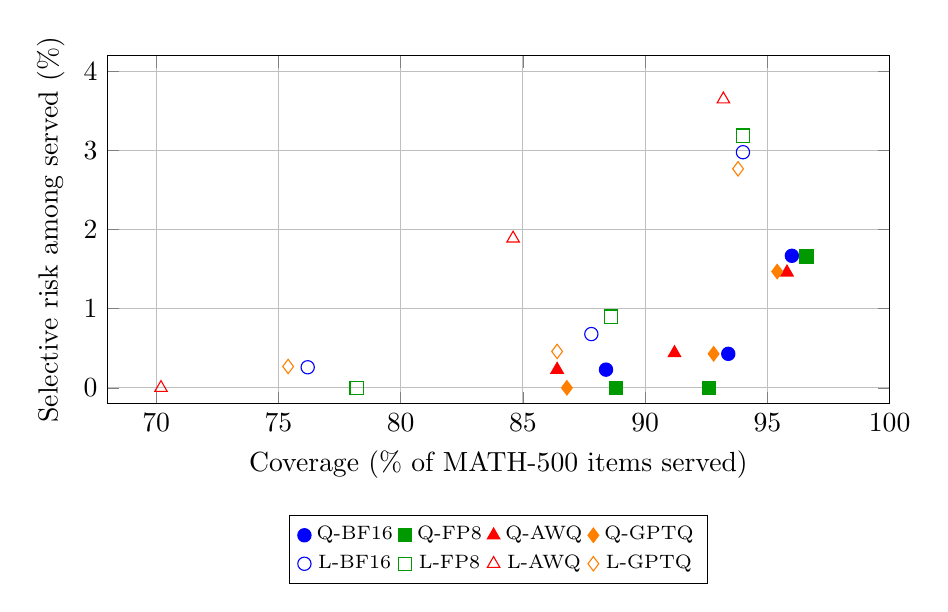
\begin{tikzpicture}
\begin{axis}[
    width=0.95\linewidth, height=6.0cm,
    xlabel={Coverage (\% of MATH-500 items served)},
    ylabel={Selective risk among served (\%)},
    xmin=68, xmax=100,
    ymin=-0.2, ymax=4.2,
    grid=major,
    legend columns=4,
    legend style={font=\scriptsize, at={(0.5,-0.32)}, anchor=north},
]
\addplot[only marks, mark=*, blue, mark size=2.4pt] coordinates {(96.0,1.67)(93.4,0.43)(88.4,0.23)};
\addplot[only marks, mark=square*, green!60!black, mark size=2.4pt] coordinates {(96.6,1.66)(92.6,0.00)(88.8,0.00)};
\addplot[only marks, mark=triangle*, red, mark size=2.6pt] coordinates {(95.8,1.46)(91.2,0.44)(86.4,0.23)};
\addplot[only marks, mark=diamond*, orange, mark size=2.6pt] coordinates {(95.4,1.47)(92.8,0.43)(86.8,0.00)};
\addplot[only marks, mark=o, blue, mark size=2.4pt] coordinates {(94.0,2.98)(87.8,0.68)(76.2,0.26)};
\addplot[only marks, mark=square, green!60!black, mark size=2.4pt] coordinates {(94.0,3.19)(88.6,0.90)(78.2,0.00)};
\addplot[only marks, mark=triangle, red, mark size=2.6pt] coordinates {(93.2,3.65)(84.6,1.89)(70.2,0.00)};
\addplot[only marks, mark=diamond, orange, mark size=2.6pt] coordinates {(93.8,2.77)(86.4,0.46)(75.4,0.27)};
\legend{Q-BF16, Q-FP8, Q-AWQ, Q-GPTQ, L-BF16, L-FP8, L-AWQ, L-GPTQ}
\end{axis}
\end{tikzpicture}
\caption{Three discrete MATH-500 operating points ($\ge 3/5$, $\ge 4/5$, $5/5$), not a continuous risk--coverage curve. Filled markers: Qwen-7B. Open markers: Llama-8B. Lower-right is high coverage and higher residual risk; lower-left is strict consensus.}
\label{fig:modal}
\end{figure}

\begin{figure}[t]
\centering
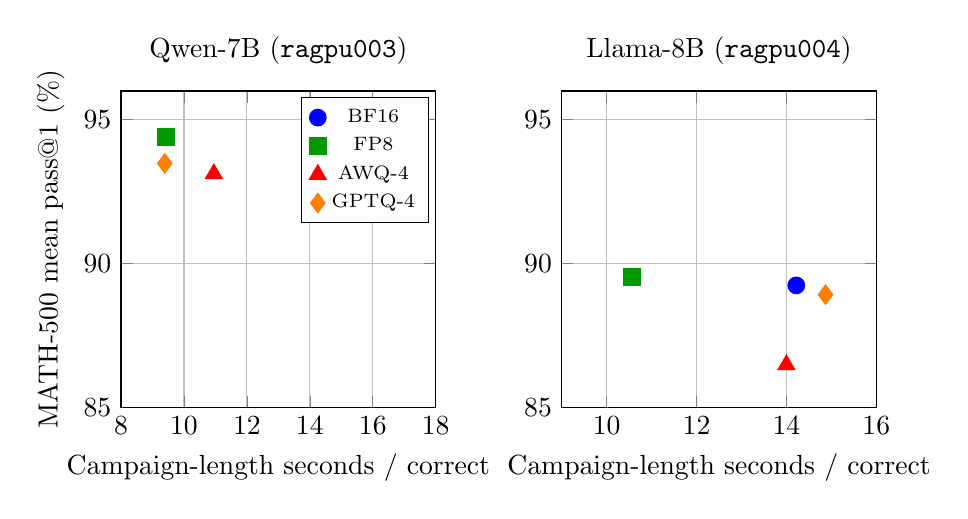
\begin{tikzpicture}
\begin{groupplot}[
    group style={
        group size=2 by 1,
        horizontal sep=1.6cm,
        ylabels at=edge left,
    },
    width=0.46\linewidth, height=5.6cm,
    xlabel={Campaign-length seconds / correct},
    ylabel={MATH-500 mean pass@1 (\%)},
    ymin=85, ymax=96,
    grid=major,
    legend style={font=\scriptsize},
]
\nextgroupplot[title={Qwen-7B (\texttt{ragpu003})}, xmin=8, xmax=18]
\addplot[only marks, mark=*, blue, mark size=3pt] coordinates {(16.89,94.00)};
\addplot[only marks, mark=square*, green!60!black, mark size=3pt] coordinates {(9.44,94.40)};
\addplot[only marks, mark=triangle*, red, mark size=3.5pt] coordinates {(10.95,93.12)};
\addplot[only marks, mark=diamond*, orange, mark size=3.5pt] coordinates {(9.39,93.48)};
\legend{BF16, FP8, AWQ-4, GPTQ-4}
\nextgroupplot[title={Llama-8B (\texttt{ragpu004})}, xmin=9, xmax=16]
\addplot[only marks, mark=*, blue, mark size=3pt] coordinates {(14.22,89.24)};
\addplot[only marks, mark=square*, green!60!black, mark size=3pt] coordinates {(10.56,89.52)};
\addplot[only marks, mark=triangle*, red, mark size=3.5pt] coordinates {(14.00,86.48)};
\addplot[only marks, mark=diamond*, orange, mark size=3.5pt] coordinates {(14.87,88.92)};
\end{groupplot}
\end{tikzpicture}
\caption{Campaign-length seconds per correct answer versus MATH-500 pass@1. The horizontal axis is full-grid mean tokens divided by the measured Condition~B tok/s and by pass@1. There are no timing whiskers: $R=3$ or $5$ does not support a percentile interval, and those repeats do not resample length. Points are not joined. Panels are separate hosts and are not a pooled trade-off plot.}
\label{fig:condB-scatter}
\end{figure}

\begin{figure}[t]
\centering
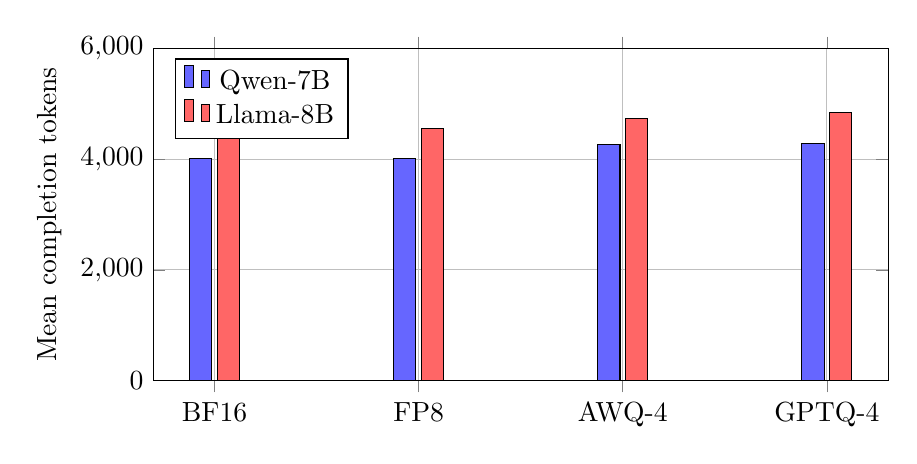
\begin{tikzpicture}
\begin{axis}[
    ybar, bar width=8pt,
    width=0.9\linewidth, height=5.8cm,
    ylabel={Mean completion tokens},
    symbolic x coords={BF16, FP8, AWQ-4, GPTQ-4},
    xtick=data,
    ymin=0, ymax=6000,
    legend pos=north west,
    grid=major,
]
\addplot[fill=blue!60] coordinates {(BF16,4011) (FP8,4008) (AWQ-4,4265) (GPTQ-4,4287)};
\addplot[fill=red!60] coordinates {(BF16,4657) (FP8,4551) (AWQ-4,4737) (GPTQ-4,4841)};
\legend{Qwen-7B, Llama-8B}
\end{axis}
\end{tikzpicture}
\caption{Full-grid mean MATH-500 completion tokens (ratio-of-means estimand). Bars are point estimates. Item-level 95\% intervals on paired token $\Delta$ are in Table~\ref{tab:tokens} and are not drawn on this axis.}
\label{fig:tokens}
\end{figure}

\begin{figure}[t]
\centering
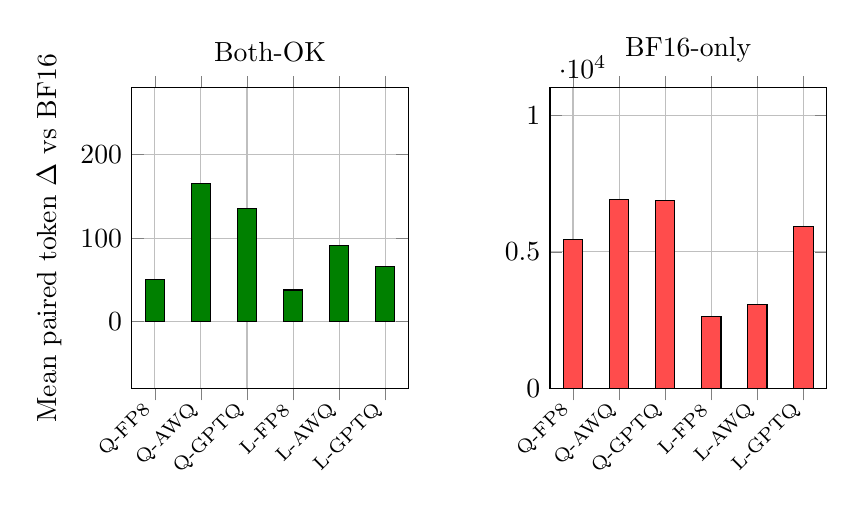
\begin{tikzpicture}
\begin{groupplot}[
    group style={
        group size=2 by 1,
        horizontal sep=1.8cm,
        ylabels at=edge left,
    },
    ybar,
    width=0.42\linewidth,
    height=5.4cm,
    symbolic x coords={Q-FP8, Q-AWQ, Q-GPTQ, L-FP8, L-AWQ, L-GPTQ},
    xtick=data,
    x tick label style={font=\scriptsize, rotate=45, anchor=east},
    grid=major,
]
\nextgroupplot[
    title={Both-OK},
    ylabel={Mean paired token $\Delta$ vs BF16},
    ymin=-80, ymax=280,
    bar width=7pt,
]
\addplot[fill=green!50!black] coordinates {(Q-FP8,51) (Q-AWQ,166) (Q-GPTQ,136) (L-FP8,38) (L-AWQ,91) (L-GPTQ,66)};
\nextgroupplot[title={BF16-only}, ymin=0, ymax=11000, bar width=7pt]
\addplot[fill=red!70] coordinates {(Q-FP8,5444) (Q-AWQ,6915) (Q-GPTQ,6892) (L-FP8,2629) (L-AWQ,3090) (L-GPTQ,5915)};
\end{groupplot}
\end{tikzpicture}
\caption{Paired token deltas by correctness, two panels so Both-OK is visible. Left: jointly-correct pairs (Qwen AWQ/GPTQ CIs exclude 0; FP8 and Llama CIs include 0; $n$ in Table~\ref{tab:tokens}). Right: BF16-correct / quantized-wrong pairs. Clustered 95\% CIs and $n$ are in Table~\ref{tab:tokens}.}
\label{fig:strata}
\end{figure}

\begin{figure}[t]
\centering
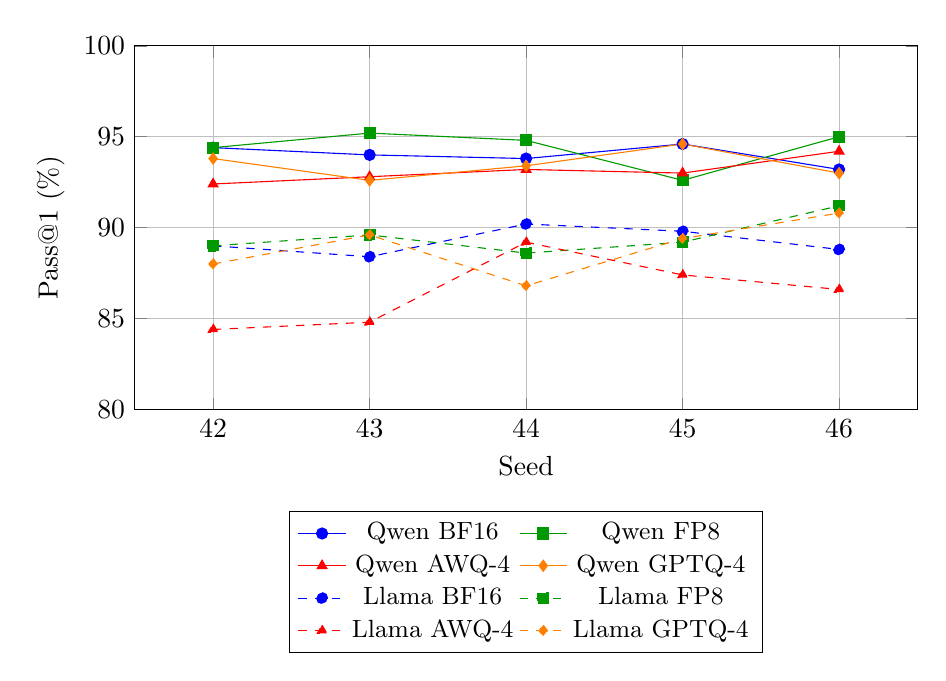
\begin{tikzpicture}
\begin{axis}[
    width=0.95\linewidth, height=6.2cm,
    xlabel={Seed},
    ylabel={Pass@1 (\%)},
    xmin=41.5, xmax=46.5,
    ymin=80, ymax=100,
    xtick={42,43,44,45,46},
    legend columns=2,
    legend style={font=\small, at={(0.5,-0.28)}, anchor=north},
    grid=major,
]
\addplot[blue, mark=*] coordinates {(42,94.4)(43,94.0)(44,93.8)(45,94.6)(46,93.2)};
\addplot[green!60!black, mark=square*] coordinates {(42,94.4)(43,95.2)(44,94.8)(45,92.6)(46,95.0)};
\addplot[red, mark=triangle*] coordinates {(42,92.4)(43,92.8)(44,93.2)(45,93.0)(46,94.2)};
\addplot[orange, mark=diamond*] coordinates {(42,93.8)(43,92.6)(44,93.4)(45,94.6)(46,93.0)};
\addplot[blue, dashed, mark=*] coordinates {(42,89.0)(43,88.4)(44,90.2)(45,89.8)(46,88.8)};
\addplot[green!60!black, dashed, mark=square*] coordinates {(42,89.0)(43,89.6)(44,88.6)(45,89.2)(46,91.2)};
\addplot[red, dashed, mark=triangle*] coordinates {(42,84.4)(43,84.8)(44,89.2)(45,87.4)(46,86.6)};
\addplot[orange, dashed, mark=diamond*] coordinates {(42,88.0)(43,89.6)(44,86.8)(45,89.4)(46,90.8)};
\legend{Qwen BF16, Qwen FP8, Qwen AWQ-4, Qwen GPTQ-4, Llama BF16, Llama FP8, Llama AWQ-4, Llama GPTQ-4}
\end{axis}
\end{tikzpicture}
\caption{MATH-500 pass@1 by seed. Solid: Qwen-7B. Dashed: Llama-8B. The tested Llama AWQ-4 checkpoint shows the largest MATH-500 pass@1 drop among the evaluated Llama cells.}
\label{fig:seed}
\end{figure}

\subsection{Measured serving throughput and Cost-of-Pass}
\label{sec:serving-results}
Table~\ref{tab:serving-main} separates tok/s from GPU-seconds per query. GPU-seconds equal output tokens divided by tok/s, so a long subset draw raises cost even when the kernel is faster. Multiplying the printed tok/s by GPU-s/q recovers the subset length. Llama FP8 Condition~A is about $7{,}288$ tokens per query. The same checkpoint's campaign mean is $4{,}550.8$, which is $2.3\%$ shorter than Llama BF16. That single 20-prompt draw, not a slower kernel, is why Condition~A ranks Llama BF16 cheapest ($\$0.0310$ vs.\ about $\$0.043$). Llama GPTQ-4 Condition~B tok/s is $0.2\%$ below BF16 ($366.16$ vs.\ $366.98$) while hybrid cost is $+24.9\%$; the gap is mostly length.

The brackets in Table~\ref{tab:serving-main} are the minimum and maximum hybrid cost across timing repeats, with campaign pass@1 held fixed. They are not a 95\% interval. Repeats share seed $20260816$, so they do not include length variance. Qwen BF16 Condition~A tok/s runs only from $43.88$ to $43.96$. Qwen FP8 Condition~B runs from $350.68$ to $546.26$, and its dollar min--max is $\$0.0030$--$\$0.0047$. Qwen FP8 Condition~B tok/s of $449.79$ is the mean of five ratios. Mean GPU-s/q is $8.64$, and $3{,}738/8.64 \approx 432.5$ tok/s. The two aggregations are not the same. Appendix Table~\ref{tab:fp8-reps} lists the five repeats. Llama FP8 and AWQ-4 Condition~A means both round to $\$0.0431$. Their repeat ranges do not: $\$0.0421$--$\$0.0449$ and $\$0.0423$--$\$0.0463$.

Table~\ref{tab:length-cost} substitutes campaign mean tokens for the subset length and keeps the measured tok/s. Under that sensitivity, Qwen GPTQ-4 is cheapest on Condition~A and tied with FP8 on Condition~B, so the AWQ/GPTQ reversal between A and B disappears. Llama FP8 is cheapest on both conditions and on mean tokens divided by pass@1. An item bootstrap of campaign tokens and pass@1, with tok/s held fixed ($B=10{,}000$), gives Llama FP8 rank~1 on both campaign-length costs in all $10{,}000$ draws. Qwen GPTQ-4 is rank~1 on Condition~A in $99.9\%$ of draws and on Condition~B in $59.6\%$, with FP8 taking the other $40.4\%$. Kendall's $\tau$ between the Qwen pass@1 order and the Condition~A campaign-length order is $-0.33$. Measured tok/s still depends on the subset's length, so Table~\ref{tab:length-cost} is not a final serving measurement. Figure~\ref{fig:condB-scatter} plots the Condition~B campaign-length seconds, not the subset dollars.

Qwen BF16 decodes at $43.92$ tok/s on Condition~A and $205.41$ tok/s in the fixed-512 microbenchmark. Llama BF16, on the other host, reaches $72.34$ and $362.01$. The fixed-length gap remains, so it is not the Condition~A length draw. Every Qwen saving in Table~\ref{tab:serving-main} ($-36.0\%$ to $-45.9\%$) is relative to that Qwen BF16 baseline on \texttt{ragpu003}. The Qwen FP8 slow/mid/fast regimes were also on that host. Clocks were not logged. AWQ-4 used the GEMM \texttt{awq} kernel rather than \texttt{awq\_marlin}. On A100 the Marlin path is the one vLLM usually selects, and it is typically faster, so every AWQ throughput number is a kernel choice as well as a format property. That choice can contribute to Llama AWQ-4 decoding more slowly than BF16 on Condition~A ($70.20$ vs.\ $72.34$ tok/s). GPTQ-4 timing used \texttt{float16} while GPTQ-4 pass@1 used \texttt{bfloat16}, so the hybrid ratio joins two configurations. These FP8 numbers are A100 Marlin W8A16, not Hopper W8A8. Peak allocated VRAM is $53.9$--$56.1$\,GB, the $0.75$ engine pool. Condition~A latency is in Appendix Table~\ref{tab:serving-single}.

\begin{table*}[t]
\centering
\caption{Hybrid cost on the controlled confirmation. Condition~A: 20 sequential prompts. Condition~B: 100-prompt \texttt{llm.generate}, \texttt{max\_num\_seqs=8}. Tok/s is mean$\pm$ sample SD. Brackets are the minimum and maximum hybrid cost across timing repeats, with campaign pass@1 held fixed. They are not a 95\% interval. The B $\Delta$\% column is the point estimate only. Qwen: \texttt{ragpu003}. Llama: \texttt{ragpu004}. GPTQ dollars join \texttt{float16} timing with \texttt{bfloat16} pass@1.}
\label{tab:serving-main}
\small
\resizebox{\textwidth}{!}{%
\begin{tabular}{llccccccc}
\toprule
\textbf{Model} & \textbf{Fmt} & \textbf{A tok/s} & \textbf{A GPU-s/q} & \textbf{A $\widetilde{C}$ [min, max]} & \textbf{B tok/s} & \textbf{B GPU-s/q} & \textbf{B $\widetilde{C}$ [min, max]} & \textbf{B $\Delta$\%} \\
\midrule
Qwen-7B & BF16   & $43.92\pm 0.04$ & 102.51 & \$0.0454 [0.0454, 0.0455] & $252.72\pm 0.56$ & 13.44 & \$0.0060 [0.0059, 0.0060] & anchor \\
Qwen-7B & FP8    & $62.50\pm 0.08$ & 84.60 & \$0.0373 [0.0373, 0.0374] & $449.79\pm 97.53$ & 8.64 & \$0.0038 [0.0030, 0.0047] & $-36.0$ \\
Qwen-7B & AWQ-4  & $76.89\pm 0.70$ & 48.04 & \$0.0215 [0.0213, 0.0217] & $418.15\pm 2.03$ & 7.82 & \$0.0035 [0.0035, 0.0035] & $-41.3$ \\
Qwen-7B & GPTQ-4 & $82.67\pm 0.69$ & 54.39 & \$0.0242 [0.0241, 0.0245] & $488.26\pm 0.64$ & 7.23 & \$0.0032 [0.0032, 0.0032] & $-45.9$ \\
\midrule
Llama-8B & BF16   & $72.34\pm 0.27$ & 66.43 & \$0.0310 [0.0309, 0.0311] & $366.98\pm 1.90$ & 10.13 & \$0.0047 [0.0047, 0.0048] & anchor \\
Llama-8B & FP8    & $78.75\pm 2.89$ & 92.55 & \$0.0431 [0.0421, 0.0449] & $481.42\pm 1.36$ & 9.32 & \$0.0043 [0.0043, 0.0044] & $-8.2$ \\
Llama-8B & AWQ-4  & $70.20\pm 2.71$ & 89.51 & \$0.0431 [0.0423, 0.0463] & $391.11\pm 0.48$ & 11.63 & \$0.0056 [0.0056, 0.0056] & $+18.5$ \\
Llama-8B & GPTQ-4 & $63.49\pm 0.41$ & 86.95 & \$0.0407 [0.0405, 0.0410] & $366.16\pm 0.79$ & 12.60 & \$0.0059 [0.0059, 0.0059] & $+24.9$ \\
\bottomrule
\end{tabular}%
}
\end{table*}

\begin{table}[t]
\centering
\caption{Campaign-length seconds per correct answer: full-grid mean MATH-500 tokens $\div$ measured tok/s $\div$ pass@1. Tok/s is the confirmation mean and is held fixed. Lower is cheaper. This is a sensitivity to subset length, not a replacement for Table~\ref{tab:serving-main}.}
\label{tab:length-cost}
\small
\begin{tabular}{llcccc}
\toprule
\textbf{Model} & \textbf{Fmt} & \textbf{A sec.} & \textbf{A rank} & \textbf{B sec.} & \textbf{B rank} \\
\midrule
Qwen-7B & BF16 & 97.16 & 4 & 16.89 & 4 \\
Qwen-7B & FP8 & 67.93 & 3 & 9.44 & 2 \\
Qwen-7B & AWQ-4 & 59.57 & 2 & 10.95 & 3 \\
Qwen-7B & GPTQ-4 & 55.48 & 1 & 9.39 & 1 \\
Llama-8B & BF16 & 72.13 & 2 & 14.22 & 3 \\
Llama-8B & FP8 & 64.55 & 1 & 10.56 & 1 \\
Llama-8B & AWQ-4 & 78.02 & 3 & 14.00 & 2 \\
Llama-8B & GPTQ-4 & 85.74 & 4 & 14.87 & 4 \\
\bottomrule
\end{tabular}
\end{table}

\FloatBarrier

\section{Discussion}
Llama AWQ-4 is the accuracy result that survives the item-level intervals on both MATH-500 and GSM8K. maj@5 removes the Qwen AWQ-4 pass@1 gap and about half of the Llama AWQ-4 gap. The BF16-correct length column is positive in every contrast because it includes quantized failures. The quant-correct column flips that sign in four of six contrasts, and three of those intervals exclude zero (Table~\ref{tab:tokens}). Both columns are selection effects.

Five-sample agreement has selective risk at most $0.27\%$. A one-sample length rule at matched coverage is higher (Table~\ref{tab:length-abstain}). The five-sample rule earns that lower risk at about five times the tokens.

Subset GPU-seconds and campaign-length seconds do not share a point order. Llama FP8 is cheapest on the campaign-length estimator in every item resample. The subset order is a property of one 20-prompt draw. Timing min--max does not cover that draw. AWQ throughput also depends on the GEMM kernel, and Qwen savings are relative to a BF16 baseline on \texttt{ragpu003}. A point order among tied cells is not evidence that bit-width has a stable deployment ranking.

\begin{table*}[t]
\centering
\caption{Practitioner summary. pass@1 and maj@5 are MATH-500 percent. Tokens are the campaign mean. A\$ and B\$ are $\widetilde{C}_{\mathrm{pass}}^{\mathrm{hyb}}$. A sec.\ and B sec.\ are the campaign-length sensitivity. $^{*}$ marks the Holm-significant MATH or GSM8K pass@1 contrast.}
\label{tab:summary}
\small
\resizebox{\textwidth}{!}{%
\begin{tabular}{llcccccc}
\toprule
\textbf{Model} & \textbf{Fmt} & \textbf{pass@1} & \textbf{maj@5} & \textbf{Tokens} & \textbf{A \$} & \textbf{B \$} & \textbf{A / B sec.} \\
\midrule
Qwen-7B & BF16 & 94.00 & 94.4 & 4{,}011 & 0.0454 & 0.0060 & 97.2 / 16.9 \\
Qwen-7B & FP8 & 94.40 & 95.0 & 4{,}008 & 0.0373 & 0.0038 & 67.9 / 9.4 \\
Qwen-7B & AWQ-4 & 93.12 & 94.4 & 4{,}265 & 0.0215 & 0.0035 & 59.6 / 11.0 \\
Qwen-7B & GPTQ-4 & 93.48 & 94.0 & 4{,}287 & 0.0242 & 0.0032 & 55.5 / 9.4 \\
Llama-8B & BF16 & 89.24 & 91.2 & 4{,}657 & 0.0310 & 0.0047 & 72.1 / 14.2 \\
Llama-8B & FP8 & 89.52 & 91.0 & 4{,}551 & 0.0431 & 0.0043 & 64.6 / 10.6 \\
Llama-8B & AWQ-4$^{*}$ & 86.48 & 89.8 & 4{,}737 & 0.0431 & 0.0056 & 78.0 / 14.0 \\
Llama-8B & GPTQ-4 & 88.92 & 91.2 & 4{,}841 & 0.0407 & 0.0059 & 85.7 / 14.9 \\
\bottomrule
\end{tabular}%
}
\end{table*}

\section{Limitations}
\begin{enumerate}
    \item \textbf{A100 W8A16 fallback.} FP8 checkpoints were executed as Marlin W8A16 on A100, not native W8A8. Numbers do not transfer to Hopper native W8A8.
    \item \textbf{Measured serving scope.} Throughput and GPU-seconds are measured on balanced MATH-500 subsets, not the full campaign. Repeats share one sampling seed, so cost intervals omit length variance. Condition~B elapsed time includes the straggler tail; occupancy time was not stored. $R=3$ or $5$ does not support a stable percentile interval. Eager execution was not compared with CUDA graphs. Qwen and Llama used different hosts, and clocks were not logged. The $\$1.50$/A100-hour rate is a pricing scenario. Peak VRAM is the $0.75$ engine pool.
    \item \textbf{Activation dtype.} AWQ-4 accuracy runs use \texttt{float16}. BF16, FP8, and accuracy-campaign GPTQ-4 use \texttt{bfloat16}. Serving GPTQ-4 uses \texttt{float16}. No BF16-at-\texttt{float16} control was run.
    \item \textbf{Pathology metrology.} The loop detector is identical-word runs $\ge 20$. Phrase-level cycles and \texttt{finish\_reason} were not saved. A chat-template recount flags 40 MATH-500 rows and 31 GSM8K rows at $32{,}768$ minus the prompt. That recount uses re-encoded completion length, which can disagree with vLLM's token count. GPQA prompts were not reconstructed, because the letter order is a process-RNG draw.
    \item \textbf{Modal agreement.} Five generations are required per attempted MATH problem. Only MATH-500 has five seeds in this campaign. Mathematical answer equivalence is evaluator- and task-specific (campaign LightEval~0.8.0 / math-verify). High agreement can still be wrong. The signal is not general uncertainty calibration, not softmax calibration, and not a safety property.
    \item \textbf{Checkpoint provenance.} Both AWQ-4 checkpoints are \texttt{jakiAJK} uploads with unknown calibration. FP8 and GPTQ-4 are RedHatAI artifacts. Format, publisher, and toolchain are collinear. No second AWQ artifact was quantized in this study.
    \item \textbf{Scope.} Two 7--8B DeepSeek-R1 distillations, English math/science, one pinned serving stack, one prompt. GSM8K/GPQA use three seeds.
    \item \textbf{Not evaluated.} This study does not evaluate AIME, LiveCodeBench, 32B models, Hopper native W8A8 FP8, energy measurements, production continuous batching, or probability calibration.
    \item \textbf{Reproducibility surface.} Compact JSON, recovered MATH-500 answer strings, confirmation timing, and analysis reports are released. Full chain-of-thought traces are not. Compact JSON omits \texttt{finish\_reason} and output token IDs. Replay needs an A100-80GB, the listed weights, and \path{runtime_manifest.json}. The driver is UNRECORDED. New sensitivities are recomputed by \path{scripts/analysis/manuscript_sensitivities.py}.
    \item \textbf{Contamination.} MATH and GSM8K overlap public pretraining corpora. A paired within-item design reduces but does not eliminate contamination interaction with checkpoint.
    \item \textbf{Launcher record.} Effective flags, including \texttt{max\_model\_len=32768}, are reconstructed in \path{runtime_manifest.json} from the launcher. They are not per-job telemetry. The NVIDIA driver is recorded as UNRECORDED. Historical harness configs are not the campaign stack.
\end{enumerate}

\paragraph{Threats to validity.}
Construct: pass@1, maj@5, token length, subset GPU-seconds, and campaign-length seconds are distinct estimands. The hybrid proxy is not Erol et al.'s per-problem Cost-of-Pass. Internal: Conditions~A and~B differ in subset and regime together; timing repeats do not resample length; Qwen and Llama used different hosts. External: two 7--8B families, one eager A100 stack, and three English benchmarks. Results do not transfer to CUDA-graph serving, Hopper W8A8, or a different publisher's AWQ artifact.

\section{Conclusion}
Under this pinned A100 / vLLM~0.7.0 eager stack, the defensible results are a selection effect in the BF16-correct length estimator, a subset serving cost that one length draw can reorder, and one robust accuracy drop. Llama AWQ-4 falls $-2.76$\,pp on MATH-500; maj@5 cuts that gap to about $-1.4$\,pp. Gold-free 5/5 agreement has selective risk at most $0.27\%$, against $1.6$--$4.6\%$ for a one-sample length rule at matched coverage. The quant-correct length mirror does not keep the sign of the BF16-correct column. Llama FP8 is cheapest once campaign length replaces the 20-prompt draw. AWQ-4 results are properties of the \texttt{jakiAJK} artifacts, run in \texttt{float16} on the GEMM \texttt{awq} kernel. GPQA letter order is not a certified paired contrast.

\section*{Reproducibility and Artifact Availability}
The released artifact enables verification of reported analyses; reproducing the complete GPU campaign requires equivalent hardware and checkpoint availability.

CPU-reproducible from compact JSON: tables, analysis scripts, and \path{scripts/analysis/manuscript_sensitivities.py} (see \path{REPRODUCE.md}). Replay of the 88-run campaign requires an NVIDIA A100-80GB, the listed weights, and \path{results/reports/runtime_manifest.json}. The driver version was not archived. Full chain-of-thought traces are not released.

Code, patches, validation JSON, and analysis reports:
\href{https://github.com/Manish06N/reasoning-compression-lab}{\nolinkurl{Manish06N/reasoning-compression-lab}}.
Per-cell records: \texttt{results/math500/}, \texttt{results/gsm8k/}, \texttt{results/gpqa/}.
Canonical pass@1 tables: \path{revision_reanalysis_report.json}.
Modal agreement: \path{modal_agreement_report.json}.
Measured serving (confirmation): \path{results/reports/measured_serving_confirmation/}.
First unconstrained timing (provenance only): \path{results/measured_serving/}. See \path{paper/ARTIFACT.md}. GPQA is a gated benchmark; public records must not republish item text.

\section*{Acknowledgment}
PARAM Rudra HPC at IIT Patna (National Supercomputing Mission, C-DAC) provided compute.

\section*{CRediT authorship contribution statement}
\textbf{Manish Nandish:} Conceptualization, Methodology, Software, Investigation, Data curation, Formal analysis, Visualization, Writing -- original draft, Writing -- review \& editing.
\textbf{Rajiv Misra:} Conceptualization, Resources, Supervision, Writing -- review \& editing.
\textbf{Midhunchakkaravarthy Janarthanan:} Supervision, Writing -- review \& editing.

The first author's dual affiliation (IIT Patna and Lincoln University College) reflects a joint doctoral arrangement. Computational experiments, software, and formal analysis were performed by Manish Nandish. No experimental or software roles are claimed for Midhunchakkaravarthy Janarthanan.

\appendix
\section{Prompt}
\label{sec:prompt}
MATH-500 and GSM8K use the QRM template. Official \texttt{inference.py} calls LightEval with \texttt{use\_chat\_template=True}:
\begin{verbatim}
{question}

Please reason step by step, and put your final
answer within \boxed{}.
\end{verbatim}
The prompt-cap recount applies that string through each family's chat template, including the generation prompt. Saved completions also begin with \texttt{<think>}; we did not insert that marker as a separate prefix.
GPQA-Diamond uses a different function in QRM's \path{lighteval_custom/tasks/reasoning.py}. The prompt asks for a final line \texttt{Answer: \$LETTER} and inserts the correct choice with \texttt{random.randint(0, 3)}. \texttt{inference.py} seeds Python's RNG with the generation seed, then loads the model, then builds prompts. The pipeline's later \texttt{random.seed(1234)} runs only after those prompts exist. Model load can consume RNG draws, and AWQ and BF16 do not take the same init path, so the letter sequence is not certified to match across checkpoints. Stored GPQA rows agree with that template: $4{,}746$ of $4{,}752$ completions contain no \texttt{\textbackslash boxed}, while pass@1 is about $41$--$53\%$ in every format, including BF16. Extractive match on GPQA is a letter match, not a boxed-answer grade. The QRM comparison row for GPQA in Table~\ref{tab:qrm-compare} is therefore not a paired contrast.

\section{Checkpoints}
\begin{table}[t]
\centering
\caption{Public checkpoints and revisions used for the 56k campaign.}
\label{tab:checkpoints}
{\footnotesize
\begin{tabular}{lp{0.72\textwidth}}
\toprule
\textbf{Cell} & \textbf{Hugging Face ID / revision} \\
\midrule
Qwen BF16 & \texttt{deepseek-ai/DeepSeek-R1-Distill-Qwen-7B}\\
 & \texttt{916b56a44061fd5cd7d6a8fb632557ed4f724f60} \\
Qwen FP8 & \texttt{RedHatAI/DeepSeek-R1-Distill-Qwen-7B-FP8-dynamic}\\
 & \texttt{ceb2fcd178d477cd21b92ffb43164c74165a212c} \\
Qwen AWQ-4 & \texttt{jakiAJK/DeepSeek-R1-Distill-Qwen-7B\_AWQ}\\
 & \texttt{1d082b3ded4e7cefbb6b32cd5e07c7d409832816} \\
Qwen GPTQ-4 & \texttt{RedHatAI/DeepSeek-R1-Distill-Qwen-7B-quantized.w4a16}\\
 & \texttt{9559a91ed463eecda64b93a532fe5aa8cc25f2eb} \\
Llama BF16 & \texttt{deepseek-ai/DeepSeek-R1-Distill-Llama-8B}\\
 & \texttt{6a6f4aa4197940add57724a7707d069478df56b1} \\
Llama FP8 & \texttt{RedHatAI/DeepSeek-R1-Distill-Llama-8B-FP8-dynamic}\\
 & \texttt{5d548d9169c53b7bb7ef0b3bc261509d5da6e3dd} \\
Llama AWQ-4 & \texttt{jakiAJK/DeepSeek-R1-Distill-Llama-8B\_AWQ}\\
 & \texttt{57360e84a0e7278c6b3abb453f2dc812b213badb} \\
Llama GPTQ-4 & \texttt{RedHatAI/DeepSeek-R1-Distill-Llama-8B-quantized.w4a16}\\
 & \texttt{faa06ed0a4a5bdab76c4df12376e0c5228c0bdfe} \\
\bottomrule
\end{tabular}
}
\end{table}

AWQ-4 checkpoints are third-party community uploads; calibration corpus and quantization code revision are unknown. GPTQ-4 and FP8 are RedHatAI compressed-tensors artifacts. This study evaluates those public checkpoints under the dtypes in Table~\ref{tab:dtype} and does not report Red Hat production serving measurements. Dataset revision SHAs are in \path{results/reports/runtime_manifest.json}.

Serving confirmation protocol and raw JSON live under \path{docs/MEASURED_SERVING_CONFIRMATION_PROTOCOL.md} and \path{results/measured_serving_confirmation/raw/}. Aggregates: \path{measured_serving_confirmation_report.json}. An earlier unconstrained timing (\path{docs/MEASURED_SERVING_PROTOCOL.md}, \path{results/measured_serving/}) is provenance only and is not mixed with confirmation means.

\section{Reanalysis}
Pathology, the item-level bootstrap, and token strata are produced by the canonical reanalysis script from the released per-cell JSON. Loop threshold $=20$. Near-cap threshold $=32{,}500$. Bootstrap $B=10{,}000$, seed $0$.

\section{Modal-agreement details}
\label{app:modal}
The compact recovered artifact has 20{,}000 rows (SHA256 prefix \texttt{23e9ead021111959}; full digest is in the JSON sidecar). It stores extracted prediction representations, campaign \path{extractive_match}, and completion tokens. It does not store chain-of-thought or problem text. Campaign extraction used LightEval~0.8.0. Campaign extractive match was reproduced on 20{,}000/20{,}000 rows before clustering. Equivalence clustering reported 0 symmetry violations, 0 transitivity violations, and 116 non-unique-mode ties among 4{,}000 groups. Bootstrap uses $B=10{,}000$ problem resamples with seed $20260816$. Secondary ECE/Brier scores (confidence $=m_i/5$) are in the JSON report and are not treated as a primary calibration result.

$T_5$ is the five-sample token-cost proxy: the sum of completion tokens over seeds 42--46. Mean / median / P90 $T_5$ are computed over all 500 items. Tokens per served query and tokens per correct served result use that same 500-item $T_5$ total in the numerator, so abstained queries are not free.

\begin{table*}[t]
\centering
\caption{Paired coverage $\Delta$ versus matched BF16 (percentage points). Intervals that exclude zero are marked $^*$. Selective-accuracy $\Delta$ intervals are in the machine-readable modal report.}
\label{tab:modal-paired}
\small
\begin{tabular}{llccc}
\toprule
\textbf{Contrast} & $\ge$3/5 cov.\ $\Delta$ [95\% CI] & $\ge$4/5 cov.\ $\Delta$ [95\% CI] & 5/5 cov.\ $\Delta$ [95\% CI] \\
\midrule
Qwen FP8     & $+0.6\ [-0.8,+2.0]$ & $-0.8\ [-2.2,+0.6]$ & $+0.4\ [-1.6,+2.4]$ \\
Qwen AWQ-4   & $-0.2\ [-1.8,+1.2]$ & $-2.2\ [-4.0,-0.6]^*$ & $-2.0\ [-4.4,+0.2]$ \\
Qwen GPTQ-4  & $-0.6\ [-2.0,+0.8]$ & $-0.6\ [-2.2,+1.0]$ & $-1.6\ [-4.2,+0.8]$ \\
Llama FP8    & $0.0\ [-1.8,+1.8]$ & $+0.8\ [-1.6,+3.2]$ & $+2.0\ [-1.2,+5.2]$ \\
Llama AWQ-4  & $-0.8\ [-2.8,+1.2]$ & $-3.2\ [-6.0,-0.6]^*$ & $-6.0\ [-9.4,-2.6]^*$ \\
Llama GPTQ-4 & $-0.2\ [-2.2,+1.8]$ & $-1.4\ [-3.8,+1.0]$ & $-0.8\ [-4.2,+2.6]$ \\
\bottomrule
\end{tabular}
\end{table*}

\section{Measured serving: latency, microbenchmark, FP8 repeats, and token proxy}
\label{app:serving}
Condition~A latency detail (Table~\ref{tab:serving-single}) is sequential decode of a balanced 20-prompt MATH-500 subset. Median latency is the mean of per-run medians. $R=3$ except Llama AWQ-4 ($R=5$; CV-triggered). Fixed-token microbenchmark (Table~\ref{tab:serving-micro}): 10 prompts $\times$ 512 tokens, $T=0.0$, \texttt{ignore\_eos}. Table~\ref{tab:fp8-reps} lists all five Qwen FP8 Condition~B repeats. Table~\ref{tab:economics} reports mean tokens divided by pass@1. It is not measured wall-clock.

\begin{table*}[t]
\centering
\caption{Confirmation single-stream serving (Condition~A: 20 sequential prompts). Latency columns are means of per-run median/P90. $\widetilde{C}_{\mathrm{pass}}^{\mathrm{hyb}}$ uses campaign MATH-500 pass@1 and a $\$1.50$/A100-hour scenario. Tok/s is mean$\pm$ sample SD.}
\label{tab:serving-single}
\small
\begin{tabular}{llccccc}
\toprule
\textbf{Model} & \textbf{Fmt} & \textbf{tok/s} & \textbf{Med.\ lat (s)} & \textbf{P90 lat (s)} & \textbf{GPU-s/q} & \textbf{$\widetilde{C}_{\mathrm{pass}}^{\mathrm{hyb}}$} \\
\midrule
Qwen-7B & BF16   & $43.92\pm 0.04$ & 59.19 & 244.83 & 102.51 & \$0.0454 \\
Qwen-7B & FP8    & $62.50\pm 0.08$ & 43.60 & 197.01 & 84.60 & \$0.0373 \\
Qwen-7B & AWQ-4  & $76.89\pm 0.70$ & 26.47 & 110.43 & 48.04 & \$0.0215 \\
Qwen-7B & GPTQ-4 & $82.67\pm 0.69$ & 34.78 & 67.51 & 54.39 & \$0.0242 \\
\midrule
Llama-8B & BF16   & $72.34\pm 0.27$ & 32.40 & 126.10 & 66.43 & \$0.0310 \\
Llama-8B & FP8    & $78.75\pm 2.89$ & 38.00 & 253.55 & 92.55 & \$0.0431 \\
Llama-8B & AWQ-4  & $70.20\pm 2.71$ & 40.12 & 246.14 & 89.51 & \$0.0431 \\
Llama-8B & GPTQ-4 & $63.49\pm 0.41$ & 46.31 & 242.83 & 86.95 & \$0.0407 \\
\bottomrule
\end{tabular}
\end{table*}

\begin{table}[t]
\centering
\caption{Fixed-token decode microbenchmark (10 prompts $\times$ 512 tokens). Isolates kernel decode speed from trace-length variation. Secondary to task-realistic Conditions~A/B.}
\label{tab:serving-micro}
\small
\begin{tabular}{llc}
\toprule
\textbf{Model} & \textbf{Fmt} & \textbf{Raw decode tok/s} \\
\midrule
Qwen-7B & BF16   & 205.41 \\
Qwen-7B & FP8    & 437.19 \\
Qwen-7B & AWQ-4  & 377.73 \\
Qwen-7B & GPTQ-4 & 401.19 \\
\midrule
Llama-8B & BF16   & 362.01 \\
Llama-8B & FP8    & 392.05 \\
Llama-8B & AWQ-4  & 344.04 \\
Llama-8B & GPTQ-4 & 302.54 \\
\bottomrule
\end{tabular}
\end{table}

\begin{table}[t]
\centering
\caption{Qwen-7B FP8 Condition~B: five technical repeats with identical aggregate $373{,}794$ output tokens. The tok/s column is a ratio. The mean GPU-s/q of $8.64$ implies $3{,}738/8.64 \approx 432.5$ tok/s, which is not the mean of the five ratios ($449.79$). Slow: tok/s $<400$. Fast: tok/s $>500$. The cause of the timing regimes was not identified.}
\label{tab:fp8-reps}
\small
\begin{tabular}{lcccc}
\toprule
\textbf{Rep} & \textbf{tok/s} & \textbf{GPU-s/q} & \textbf{$\widetilde{C}_{\mathrm{pass}}^{\mathrm{hyb}}$} & \textbf{Regime} \\
\midrule
1 & 350.91 & 10.6522 & \$0.0047 & slow \\
2 & 350.68 & 10.6591 & \$0.0047 & slow \\
3 & 455.90 & 8.1990 & \$0.0036 & mid \\
4 & 545.18 & 6.8563 & \$0.0030 & fast \\
5 & 546.26 & 6.8427 & \$0.0030 & fast \\
\midrule
Mean of ratios & $449.79\pm 97.53$ & 8.64 & \$0.0038 & keep all five \\
Median / IQR & 455.90 / [350.91, 545.18] & --- & --- & --- \\
\bottomrule
\end{tabular}
\end{table}

\begin{table}[t]
\centering
\caption{MATH-500 mean tokens divided by pass@1. This is the order a shared throughput would produce. It is not measured wall-clock. Primary cost evidence is Table~\ref{tab:serving-main} and Table~\ref{tab:length-cost}.}
\label{tab:economics}
\small
\begin{tabular}{lcc}
\toprule
\textbf{Cell} & \textbf{Mean tok.} & \textbf{Tokens / correct} \\
\midrule
Qwen BF16   & 4{,}011.4 & 4{,}267 \\
Qwen FP8    & 4{,}007.7 & 4{,}245 \\
Qwen AWQ-4  & 4{,}265.3 & 4{,}580 \\
Qwen GPTQ-4 & 4{,}287.2 & 4{,}586 \\
\midrule
Llama BF16   & 4{,}656.6 & 5{,}218 \\
Llama FP8    & 4{,}550.8 & 5{,}084 \\
Llama AWQ-4  & 4{,}736.5 & 5{,}477 \\
Llama GPTQ-4 & 4{,}840.5 & 5{,}443 \\
\bottomrule
\end{tabular}
\end{table}

\section{Neighboring measurement studies}
\label{app:related}
Table~\ref{tab:related} is a compact comparison. It is not a claim that this paper replaces those studies.

\begin{table*}[t]
\centering
\caption{Neighboring measurement studies. ``Engine pinned'' means one named serving stack is frozen while checkpoints vary. Length estimands and serving columns are what each paper reports as primary evidence, not an exhaustive inventory.}
\label{tab:related}
\small
\resizebox{\textwidth}{!}{%
\begin{tabular}{lcccccccc}
\toprule
\textbf{Study} & \textbf{Models} & \textbf{Bits} & \textbf{Engine pinned} & \textbf{Seeds} & \textbf{Length estimand} & \textbf{Correctness split} & \textbf{Serving / cost} & \textbf{Statistics} \\
\midrule
This paper & 2 R1 distill (7B/8B) & BF16, FP8, AWQ-4, GPTQ-4 & vLLM 0.7.0 eager, A100 & 5 MATH; 3 GSM/GPQA & RoM, paired $\Delta$, both conditionals & $2\times 2$ + both mirrors & GPU-s; campaign-length seconds & item-level bootstrap, Holm, TOST \\
QRM~\cite{liu2025qrm} & R1 distill family & W/A/KV incl.\ W4A16 & QRM harness (multi-config) & typically 1 & mean tokens & not $2\times 2$ & limited & per-cell means \\
Lian et al.~\cite{lian2026quantinflates} & reasoning PTQ & low-bit PTQ & paper stack & paper-specific & BF16-correct $\Delta$ & BF16-correct vs rest & token cost & paired length \\
Lotfi et al.~\cite{lotfi2026overthinking} & 1.5B--32B reasoning & aggressive PTQ & paper stack & paper-specific & CoT length; overthinking & abandoned intermediates & logit-penalty Pareto & error-type counts \\
Kurtic et al.~\cite{kurtic2025give} & Llama-3.1 + R1-distill & FP8/INT8/INT4 & vLLM, several GPUs & large evals & not CoT-primary & N/A & sync vs continuous batching & accuracy + tok/s \\
Helcig et al.~\cite{helcig2026slq} & Llama/Qwen (SLQ) & 3.3--6 bpp & vLLM kernels & 3 (GSM) & thinking tokens & TL vs DL fidelity & vLLM throughput & EAR, Wilcoxon \\
Erol et al.~\cite{erol2025costofpass} & general LMs & N/A & N/A & N/A & N/A & N/A & $C_{\mathrm{pass}}$ definition & economic \\
Hochlehnert et al.~\cite{hochlehnert2025sober} & reasoning LMs & N/A & deliberately \emph{un}pinned & many & N/A & N/A & N/A & reproducibility \\
\bottomrule
\end{tabular}%
}
\end{table*}

\section{Holm-18 sensitivity}
\label{app:holm18}
Primary multiplicity control is Holm--Bonferroni within each benchmark's six format contrasts. Table~\ref{tab:holm18} applies Holm jointly to all 18 contrasts as a stricter sensitivity. Llama MATH AWQ-4 and Llama GSM8K AWQ-4 remain significant. Qwen GPQA AWQ-4 does not (Holm-18 $p=0.109$). The raw bootstrap $p$ is $0.0068$.

\begin{table}[t]
\centering
\caption{Secondary Holm correction over all 18 pass@1 contrasts. Primary inference remains Holm-6 within each benchmark. sig.: Holm-significant at $\alpha=0.05$; n.s.: not significant.}
\label{tab:holm18}
\small
\begin{tabular}{llcccc}
\toprule
\textbf{Bench.} & \textbf{Contrast} & $p$ & \textbf{Holm-6} & \textbf{Holm-18 $p$} & \textbf{Holm-18} \\
\midrule
MATH & Llama AWQ-4 & $<0.001$ & sig. & $<0.001$ & sig. \\
MATH & Qwen AWQ-4 & $0.069$ & n.s. & $1.000$ & n.s. \\
MATH & Qwen GPTQ-4 & $0.245$ & n.s. & $1.000$ & n.s. \\
MATH & Qwen FP8 & $0.383$ & n.s. & $1.000$ & n.s. \\
MATH & Llama GPTQ-4 & $0.619$ & n.s. & $1.000$ & n.s. \\
MATH & Llama FP8 & $0.647$ & n.s. & $1.000$ & n.s. \\
GSM8K & Llama AWQ-4 & $0.002$ & sig. & $0.031$ & sig. \\
GSM8K & Llama GPTQ-4 & $0.511$ & n.s. & $1.000$ & n.s. \\
GSM8K & Qwen AWQ-4 & $0.579$ & n.s. & $1.000$ & n.s. \\
GSM8K & Qwen GPTQ-4 & $0.729$ & n.s. & $1.000$ & n.s. \\
GSM8K & Llama FP8 & $0.761$ & n.s. & $1.000$ & n.s. \\
GSM8K & Qwen FP8 & $0.827$ & n.s. & $1.000$ & n.s. \\
GPQA & Qwen AWQ-4 & $0.007$ & sig. & $0.109$ & n.s. \\
GPQA & Qwen GPTQ-4 & $0.288$ & n.s. & $1.000$ & n.s. \\
GPQA & Llama FP8 & $0.403$ & n.s. & $1.000$ & n.s. \\
GPQA & Llama GPTQ-4 & $0.573$ & n.s. & $1.000$ & n.s. \\
GPQA & Qwen FP8 & $0.690$ & n.s. & $1.000$ & n.s. \\
GPQA & Llama AWQ-4 & $0.711$ & n.s. & $1.000$ & n.s. \\
\bottomrule
\end{tabular}
\end{table}

\bibliographystyle{plain}
\bibliography{references}

\end{document}
